\documentclass[11pt, a4paper, oneside]{report}
\usepackage[french]{babel}
\frenchbsetup{ReduceListSpacing=false}
\usepackage[
  top=2.5cm, 
  bottom=2.5cm, 
  left=2.5cm,   % Marge gauche un peu plus large pour la reliure
  right=2.5cm   % Marge droite
]{geometry}
\usepackage[T1]{fontenc}
\usepackage{anyfontsize}
\usepackage{lmodern}
\usepackage{stackengine}
\usepackage{xfrac}
\usepackage{mathrsfs}
\usepackage{amsfonts}
\usepackage{amsmath}
\usepackage{amssymb}
\usepackage{mathtools}
\usepackage{bm}
\usepackage{dsfont}
\usepackage{cancel}
\usepackage{stmaryrd}
\usepackage{graphicx} 
\usepackage{xcolor}
\usepackage{siunitx}
\usepackage{subcaption}
\usepackage{booktabs}
\usepackage{float}
\usepackage{tikz}

\definecolor{VertFonce}{RGB}{34, 139, 34}   
\definecolor{RougeFonce}{RGB}{165, 42, 42}  
\definecolor{BleuFonce}{RGB}{30, 60, 120}   

\usepackage[
    colorlinks=true,
    linkcolor=RougeFonce,
    citecolor=VertFonce,  
    urlcolor=teal,
    breaklinks=true
]{hyperref}

\usepackage[Bjornstrup]{fncychap}

\usepackage[title, titletoc]{appendix}

\newcommand{\restricdynamic}[2]{\left.#1\right\vert_{#2}}

\newcommand{\LegendreL}{\mathfrak{L}}
\newcommand{\DubinerD}{\mathfrak{D}}

\begin{document}

\begin{titlepage}

    % --- LOGOS ---
    \begin{center}
        % Première ligne : École d'ingénieur et Universités
        
\includegraphics[height=1.8cm]{./PNG/enseirb_matmeca_logo.jpg}\hfill
        
\includegraphics[height=1.8cm]{./PNG/toulon_logo.png}\hfill
        
\includegraphics[height=1.8cm]{./PNG/la_rochelle_logo.png}
        
        \vspace{0.4cm}
        
        % Seconde ligne : Laboratoires
        
\includegraphics[height=1.8cm]{./PNG/imath_logo.png}\hspace{1cm}
        
\includegraphics[height=1.8cm]{./PNG/mia_logo.png}
    \end{center}

    \vspace{1cm}

    % --- EN-TÊTE / CONTEXTE ---
    \begin{center}
        {\Large \textsc{Rapport de stage d'application}}\\[0.6cm]
    \end{center}

    % --- TITRE DU RAPPORT (Titre et saut de ligne plus aérés) ---
    \vspace{0.5cm}
    \begin{center}
        \hrule
        \vspace{0.8cm}
        {\huge \bfseries 
            \begin{tabular}{c}
                Intégration de l'équation d'Exner dans le \\[0.3em]
                code RIVAGE en utilisant des méthodes de \\[0.3em]
                Galerkin discontinues
            \end{tabular}
        }\\[0.8cm]
        \hrule
    \end{center}

    \vspace{1.5cm}

    % --- AUTEUR ET ENCADRANTS DU MÊME CÔTÉ (À GAUCHE) ---
    \noindent
    \begin{minipage}[t]{0.8\textwidth}
        \textbf{Présenté par :} \\[0.15cm]
        Lucas \textsc{Gadbin} 
        
        \vspace{0.4cm}
        
        \textbf{Directeurs de stage :} \\
        M. Mehmet \textsc{Ersoy} -- Professeur des universités -- Université de Toulon \\[0.1cm]
        Mme. Catherine \textsc{Choquet} -- Professeure des universités -- Université de La Rochelle \\[0.25cm]
        \textbf{Co-encadrant :} \\
        M. Yolhan \textsc{Mannes} -- Post-doctorant -- Laboratoire IMATH

        \vspace{0.4cm}

        \textbf{Tuteur académique :} \\
        M. Julien \textsc{Moatti} -- Maître de conférences -- ENSEIRB-MATMECA
    \end{minipage}

    \vfill

    % --- PIED DE PAGE ---
    \begin{center}
        \rule{0.5\textwidth}{0.4pt}\\[0.3cm]
        Laboratoires d'accueil : IMATH \& MIA \\
        Période du stage : 30 mars au 25 septembre 2026 \\
        Année universitaire : 2025--2026
    \end{center}

\end{titlepage}

\thispagestyle{empty}
\section*{Résumé}

La simulation des écoulements côtiers présente un double intérêt environnemental et socio-économique majeur, permettant de modéliser l'érosion des plages et de prévenir les risques d'inondation des zones habitées. \\
L'équation d'Exner, qui régit l'évolution de la bathymétrie liée au transport sédimentaire, est résolue ici en 1D et 2D à l'aide de méthodes Runge-Kutta Galerkin discontinues. Cette approche se révèle particulièrement adaptée pour traiter la raideur potentielle des équations et faciliter la montée en ordre. \\
L'étude des lois empiriques du flux et la discussion du domaine d'hyperbolicité du système de Saint-Venant-Exner permettent de valider avec succès le modèle numérique face à diverses solutions manufacturées, analytiques et semi-analytiques issues de la littérature. \\
Enfin, le cadre théorique et la formulation discrète d'une approche Runge-Kutta Galerkin discontinue sont également établis pour le système couplé, posant ainsi les bases formelles de son intégration future. \\

\noindent
Mots-clés : Équations de Saint-Venant-Exner, Méthode Galerkin discontinue, Schémas IMEX, Transport sédimentaire, Écoulements côtiers

\section*{Abstract}

The simulation of coastal flows is of major environmental and socio-economic importance, enabling the modeling of beach erosion and the prevention of flooding risks in inhabited areas. \\
The Exner equation, which governs bathymetric evolution due to sediment transport, is solved here in 1D and 2D using Runge-Kutta discontinuous Galerkin methods. This approach proves particularly well-suited for handling the potential stiffness of the equations and facilitating high-order extension. \\
The study of empirical flux laws and the discussion of the hyperbolicity domain of the Saint-Venant-Exner system enable the successful validation of the numerical model against various manufactured, analytical, and semi-analytical solutions from the literature. \\
Finally, the theoretical framework and discrete formulation of a Runge-Kutta discontinuous Galerkin approach are also established for the coupled system, thereby laying the formal foundations for its future integration. \\

\noindent
Keywords : Saint-Venant-Exner equations, Discontinuous Galerkin methods, IMEX schemes, Sediment transport, Coastal flows

\tableofcontents
\thispagestyle{empty}

\chapter*{Introduction}
\addcontentsline{toc}{chapter}{Introduction}
\setcounter{page}{1}

La simulation des écoulements côtiers présente un double intérêt environnemental et socio-économique majeur : elle permet de modéliser l'érosion des plages et de prédire le risque d'inondation des zones habitées.
Ces écoulements se déroulent principalement en eaux peu profondes — où la longueur d'onde de la vague est grande devant la hauteur d'eau — et sont classiquement modélisés par les équations de Saint-Venant $(\mathcal{SW})$. Celles-ci intègrent un terme lié à la bathymétrie, dont l'évolution temporelle est quantifiée par l'équation d'Exner \eqref{eq:Exner_generalisee}. Dès lors, le couplage de ces équations devient pertinent pour simuler fidèlement la dynamique hydro-morphodynamique associée. \\

L'équation d'Exner est une équation de conservation de transport, dont le flux est régi par des lois empiriques (Grass, Meyer-Peter et Müller) faisant intervenir la vitesse de l'eau donnée par $(\mathcal{SW})$.
Obtenues en moyennant la vitesse sur la hauteur sous l'hypothèse de pression hydrostatique, les équations de Saint-Venant induisent par construction une erreur sur la contrainte au fond et faussent le flux de \eqref{eq:Exner_generalisee}. \\
Pour y pallier, plusieurs approches existent : diviser le domaine en sous-domaines de vitesse moyenne différente (modèles multi-couches \cite{bonaventura2018multilayer}), considérer une expansion polynomiale de la vitesse (modèles \textit{Hyperbolic Shallow Water Moment} \cite{kowalski2017moment,garres2020shallow,parvin2025coupled}), ou dériver un modèle enrichi par analyse asymptotique des équations de Navier-Stokes incompressibles pénalisées.
C'est le système couplé Saint-Venant-Exner \eqref{eq:Saint_Venant_Exner} issu de cette dernière approche, établi dans \cite{ba2026coupled}, que nous souhaitons résoudre numériquement dans ce stage. \\

La discrétisation spatiale de \eqref{eq:Saint_Venant_Exner} s'appuie généralement sur les Volumes Finis ou la méthode de Galerkin discontinue (DG). La première a été largement étudiée et privilégiée pour sa robustesse et son faible coût, menant jusqu'à un schéma semi-implicite d'ordre trois \cite{fernandez2025third}. De plus, la solution y étant constante par maille, la gestion des fronts mouillés/secs y est plus directe qu'en DG, où réduire la solution à un degré nul dégradait jusqu'ici sa compétitivité. \\
Toutefois, la récente approche par maille fantôme \cite{poussel2025wetting} permet désormais de traiter les mailles semi-sèches en les divisant en une partie mouillée et une partie sèche, conservant ainsi des fonctions affines plutôt que constantes.
Par conséquent, une méthode \textit{Runge-Kutta Discontinuous Galerkin} (RKDG) devient compétitive vis-à-vis d'une méthode Volumes Finis, tirant parti de son aptitude à capturer les chocs et de sa flexibilité pour monter en ordre. \\
Le code RIVAGE disposant déjà d'un solveur RKDG pour Saint-Venant, l'enjeu de ce stage est d'implémenter une résolution similaire pour l'équation d'Exner, puis d'effectuer le couplage afin d'obtenir la résolution RKDG complète du système \eqref{eq:Saint_Venant_Exner}.

\chapter{Équation d'Exner généralisée et formulation de Galerkin discontinue}

Dans ce chapitre, nous allons construire un schéma numérique RKDG pour l'équation d'Exner généralisée proposée par Ba \textit{et al.} \cite{ba2026coupled}, puis nous validerons numériquement notre implémentation sur trois cas tests. Le premier est une solution manufacturée et les deux autres sont issus de la littérature. \\
Ainsi, nous nous intéressons à la résolution du problème : trouver $b(\bm{x}, t) : \Omega \times (0, T) \longrightarrow \mathbb{R}$ tel que
\begin{equation} \tag{$\mathcal{E}$} \label{eq:Exner_generalisee}
    \left \{
    \begin{aligned}
        &m(\nabla b) \partial_t b(\bm{x}, t) + \nabla \cdot \bm{G}(b; h, \bm{u}, \tau) = S(b; h, \bm{u}, \tau)  &&\text{sur } \Omega \times (0, T) \\
        &b(\bm{x}, t) = b_D(\bm{x}, t)    &&\text{sur } \Gamma_D \times (0, T) \\
        &\bm{G}(b; h, \bm{u}, \tau) \cdot \bm{n} = \bm{q}_N(\bm{x}, t)  &&\text{sur } \Gamma_N \times (0, T) \\
        &b(\bm{x}, 0) = b_\text{ini}(\bm{x})  &&\text{sur } \Omega
    \end{aligned}
    \right .
\end{equation}
où $T$ est le temps final, $\Omega \subset \mathbb{R}^2$ est le domaine physique, $\Gamma_D$ et $\Gamma_N$ sont les frontières soumises à des conditions aux limites de Dirichlet et Neumann, $m$ est la métrique géométrique, $b$ est la hauteur de la bathymétrie, $\bm{G}$ est le flux de l'équation d'Exner et $S$ est le terme source. \\
De plus, le triplet $(h, \bm{u}, \tau)$ est issu de la résolution des équations de Saint-Venant et représente respectivement la hauteur d'eau, la vitesse du fluide et la contrainte de frottement appliquée au lit sédimentaire. \\
\begin{samepage}
Dans la formulation $\eqref{eq:Exner_generalisee}$, les différents opérateurs se définissent ainsi :
\begin{itemize}
    \item $\displaystyle m(\nabla b) = \frac{1}{\sqrt{1 + \left\| \nabla b \right\|^2}}$ caractérise la métrique géométrique issue de la formulation \textit{level-set} de l'interface
    \item $\displaystyle \bm{G}(b; h, \bm{u}, \tau) = \bm{Q}_d(b; h, \bm{u}) \mathds{1}_{\tau \leq \tau_c} + \bm{Q}_e(b; h, \bm{u}) \mathds{1}_{\tau > \tau_c}$ désigne le flux sédimentaire global associé au transport par charriage à la paroi
    \item $\displaystyle S(b, h, \bm{u}, \tau) = D(b; h, \bm{u}) \mathds{1}_{\tau \leq \tau_c} - E(b; h, \bm{u}) \mathds{1}_{\tau > \tau_c}$ est le terme source d'échange de masse par dépôt et érosion, quantifiant le transport en suspension
\end{itemize}
Cette formulation faisant intervenir des indicatrices, nous faisons le choix de les lisser au travers d'une sigmoïde définie comme
\begin{equation}
    \mathcal{S}(\tau) = \frac{1}{2} \left( 1 + \tanh \left( \frac{\tau - \tau_c}{\varepsilon_\tau} \right) \right)
\end{equation}
de telle sorte que
\begin{equation}
    \mathds{1}_{\tau \leq \tau_c} = 1 - \mathcal{S}(\tau) \quad \text{et} \quad \mathds{1}_{\tau > \tau_c} = \mathcal{S}(\tau)
\end{equation}
où $\varepsilon_\tau \in (0, \tau_c)$ est un paramètre fixé par l'utilisateur contrôlant la raideur de la transition : plus $\varepsilon_\tau$ est petit, plus les indicatrices convergent vers des fonctions de Heaviside. \\
\end{samepage}
Au-delà de l'intérêt numérique, cela permet aussi de donner plus de sens physique aux lois empiriques : en réalité on ne passe pas instantanément d'un régime de dépôt à un régime d'érosion. De fait, proche du seuil critique $\tau_c$, il est \textit{a priori} envisageable d'avoir toujours des grains qui se déposent au fond. On peut aussi considérer que cette régularisation permet de simuler des grains de taille légèrement variable : un grain de plus petit diamètre sera dans un régime d'érosion pour une contrainte plus faible que la contrainte critique $\tau_c$ associée au diamètre moyen $d_{50}$ des sédiments. \\
En ce sens, on fait le choix de fixer $\varepsilon_\tau = 0.1 \tau_c$, de telle sorte que la sigmoïde $\mathcal{S}$ effectue la quasi-totalité de sa transition de 0 à 1 sur l'intervalle $\tau \in [0.7 \tau_c, 1.3 \tau_c]$.

\section{Formulation semi-discrète}

La méthode DG peut être vue comme une méthode d'Éléments Finis (EF) pour laquelle la solution numérique peut posséder des discontinuités aux interfaces des mailles. Elle s'apparente également à une méthode de Volumes Finis (VF) où la solution est approximée de manière polynomiale sur une maille, plutôt que par une valeur constante. Pour une présentation synthétique du formalisme variationnel DG en 1D et des liens avec les méthodes EF et VF, le lecteur est invité à consulter l'annexe \ref{annexe:DG_1D}.

Considérons $\mathcal{M}^n$ un maillage conforme et non uniforme de $\Omega$ au temps $t^n$ composé de $N_e$ éléments notés $\Omega_i^n$. On note $\widehat{\Omega}$ la maille de référence et $\widehat{F} = [-1, 1]$ la face de référence. Comme on s'intéresse à des maillages non structurés de quadrilatères ou de triangles, l'élément de référence change selon la forme des mailles : si les mailles sont rectangulaires, alors
\begin{equation}
    \widehat{\Omega} = \mathcal{Q} = \left\{ (x, y) \in \mathbb{R}^2 : -1 \leq x \leq 1, ~ -1 \leq y \leq 1 \right\}
\end{equation}
et si les mailles sont triangulaires, alors
\begin{equation}
    \widehat{\Omega} = \mathcal{T} = \left\{ (x, y) \in \mathbb{R}^2 : 0 \leq x, y \leq 1, ~ 0 \leq x + y \leq 1 \right\}
\end{equation}

\begin{samepage}
Comme $\mathcal{M}^n$ est conforme, il existe une application $\widehat{\phi}_i(\xi, \eta) : \widehat{\Omega} \longrightarrow \Omega_i^n$ qui envoie l'élément de référence sur la maille $\Omega_i^n$ et son inverse $\widehat{\phi}_i^{-1}(x, y) : \Omega_i^n \longrightarrow \widehat{\Omega}$ mappant les coordonnées de la maille $\Omega_i^n$ vers l'élément de référence $\widehat{\Omega}$. \\
De plus, on introduit $\widehat{\phi}_F(\xi) : \widehat{F} \longrightarrow F$ l'application envoyant la face de référence $\widehat{F}$ sur la face physique $F$. Étant donné que nous travaillons en 2D, l'inverse de cette application n'est pas défini, mais c'est un faux problème car, en DG, les faces ne contiennent pas d'informations sur les inconnues, seules les mailles en contiennent. \\
Ainsi, on peut introduire le changement de variable d'une face $F$, de sommets de coordonnées $(x_1, y_1)$ et $(x_2, y_2)$, vers la face de référence $\widehat{F}$ : si $g : F \longrightarrow \mathbb{R}$, alors
\begin{equation}
    \int_F g(x, y) \text{d}F = \int_{\widehat{F}} g(\widehat{\phi}_F(\xi)) \lvert F \rvert \text{d}\widehat{F}
\end{equation}
avec $\lvert F \rvert = \sqrt{(x_2 - x_1)^2 + (y_2 - y_1)^2}/2$ le Jacobien du changement de variable. \\
En outre, pour une application $g : \Omega_i^n \longrightarrow \mathbb{R}$, on a
\begin{equation}
    \int_{\Omega_i^n} g(x, y) \text{d}\bm{x} = \int_{\widehat{\Omega}} g(\widehat{\phi}_i(\xi, \eta)) \lvert \Omega_i^n \rvert \text{d}\widehat{\Omega}
\end{equation}
et si $g$ est différentiable sur la maille $\Omega_i^n$, alors
\begin{equation}
    \int_{\Omega_i^n} \nabla g(x, y) \text{d}\bm{x} = \int_{\widehat{\Omega}} \widetilde{\nabla}_i g(\widehat{\phi}_i(\xi, \eta)) \lvert \Omega_i^n \rvert \text{d}\widehat{\Omega}
\end{equation}
où $\displaystyle \widetilde{\nabla}_i = \left( \mathbb{J}_i^{-1}(\xi, \eta) \right)^T \begin{pmatrix} \partial_\xi \\ \partial_\eta \end{pmatrix}$ est l'opérateur différentiel provenant de la règle de la chaîne, ${\displaystyle \lvert \Omega_i^n \rvert = \left| \det \left( \mathbb{J}_i(\xi, \eta) \right) \right|}$ le facteur de forme et $\mathbb{J}_i$ la matrice Jacobienne de $\widehat{\phi}_i$.
\end{samepage}

\begin{samepage}
Enfin, la solution approchée du problème \eqref{eq:Exner_generalisee} est cherchée sur l'espace DG étant défini par
\begin{equation}
    \mathcal{V}^\mathbf{p}(\mathcal{M}^n) = \left\{ v \in L^2(\Omega) : \restricdynamic{v}{\Omega_i^n} \in \mathbb{P}^{p_i}(\Omega_i^n), \forall \Omega_i^n \in \mathcal{M}^n \right\}
\end{equation}
où $\displaystyle \mathbb{P}^{p_i}(\Omega_i^n)$ désigne l'ensemble des polynômes de degré au plus $p_i$ sur une maille $\Omega_i^n$. \\
La base de l'espace des polynômes de degré au plus $p_i$ diffère elle aussi selon la forme des mailles. \\
D'une part, si $\Omega_i^n$ est un rectangle, alors on utilise la base de Legendre 2D, construite par produit tensoriel des polynômes de Legendre 1D, soit
\begin{equation}
    \LegendreL_{k, m}(\xi, \eta) = c_k \mathcal{L}_k(\xi) c_m \mathcal{L}_m(\eta), ~ 0 \leq k, m \leq p_i
\end{equation}
avec $\mathcal{L}_k$ le polynôme de Legendre de degré $k$ et $c_k = \sqrt{(2k+1)/2}$ sa constante de normalisation. \\
D'autre part, si $\Omega_i^n$ est un triangle, alors on utilise la base de Dubiner \cite{dubiner1991spectral}, construite à partir des polynômes de Legendre et de Jacobi, de sorte que
\begin{equation}
    \DubinerD_{k, m}(\xi, \eta) = C_{k, m} 2^k \mathcal{L}_k \left( \frac{2 \eta}{1 - \xi} - 1 \right) (1 - \xi)^k \mathcal{P}_m^{(2k+1, 0)}(2 \xi - 1), ~ 0 \leq k + m \leq p_i
\end{equation}
où $C_{k, m}$ est une constante de normalisation et $\mathcal{P}_m^{(2k+1, 0)}$ est le polynôme de Jacobi de degré $m$ et de paramètres $(2k+1, 0)$. \\
Ce choix est justifié par l'orthogonalité de ces deux bases pour le produit scalaire de $L^2(\mathcal{Q})$ et $L^2(\mathcal{T})$, ainsi que par leur caractère hiérarchique, permettant alors de choisir le degré polynomial au sein de chaque maille sans devoir générer à nouveau ces deux bases. \\
Pour finir l'introduction des notations, on note $N_\text{ddl}^i$ le nombre de degrés de liberté de la maille $\Omega_i^n$ tel que
\begin{equation}
    N_\text{ddl}^i =
    \left \{
    \begin{aligned}
        &(p_i + 1)^2                &&\text{si } \widehat{\Omega} = \mathcal{Q} \\
        &\frac{(p_i+1)(p_i+2)}{2}   &&\text{si } \widehat{\Omega} = \mathcal{T}
    \end{aligned}
    \right .
\end{equation}
Par conséquent, pour $\displaystyle v_i \in \mathbb{P}^{p_i}(\Omega_i^n)$, nous avons la combinaison linéaire
\begin{equation} \label{eq:Projection_DG}
    v_i(\bm{x}, t) = \bm{\Phi}_i^T(\bm{x}) \bm{V}_i(t)
\end{equation}
avec $\displaystyle \bm{\Phi}_i \in \mathbb{R}^{N_\text{ddl}^i}$ le vecteur contenant les fonctions de base et $\displaystyle \bm{V}_i \in \mathbb{R}^{N_\text{ddl}^i}$ le vecteur caractérisant les degrés de liberté de $v_i$. \\

L'obtention de la formulation variationnelle du problème \eqref{eq:Exner_generalisee} est en tout point semblable à une méthode EF : on multiplie l'équation d'Exner par une fonction test $\varphi \in \mathcal{V}^\mathbf{p}(\mathcal{M}^n)$ puis on intègre sur l'ensemble des mailles $\Omega_i^n$ du maillage, ce qui donne le problème
\begin{equation} \tag{$\mathcal{P}_{SD}^{\mathcal{E}}$} \label{eq:Probleme_variationnel_exner}
    \left \{
    \begin{aligned}
        & \text{Trouver } b_h \in \mathcal{V}^\mathbf{p}(\mathcal{M}^n) \text{ tel que } \forall \varphi \in \mathcal{V}^\mathbf{p}(\mathcal{M}^n) \\
        & m_\mathcal{E}^n(\partial_t b_h, \varphi; b_h) + a_\mathcal{E}^n(\varphi; b_h) = l_\mathcal{E}^n (\varphi)
    \end{aligned}
    \right .
\end{equation}
où les applications DG $m_\mathcal{E}^n$ et $a_\mathcal{E}^n$, et la forme linéaire $l_\mathcal{E}^n$ sont définies comme
\begin{equation}
    \begin{aligned}
        \forall v_1, v_2, \varphi \in \mathcal{V}^\mathbf{p}(\mathcal{M}^n), ~ &m_\mathcal{E}^n(v_1, \varphi; v_2) = \sum_{\Omega_i^n \in \mathcal{M}^n} \int_{\Omega_i^n} m(\nabla v_2) v_1 \varphi \text{d}\bm{x} \\
        & a_\mathcal{E}^n(\varphi; v_1) = - \sum_{\Omega_i^n \in \mathcal{M}^n} \int_{\Omega_i^n} \bm{G}(v_1) \cdot \nabla \varphi \text{d}\bm{x} - \sum_{\Omega_i^n \in \mathcal{M}^n} \int_{\Omega_i^n} S(v_1) \varphi \text{d}\bm{x} \\
        & \phantom{a_\mathcal{E}^n(\varphi; v_1) = } - \sum_{F \in \mathcal{F}^\text{int}} \int_F \left( \bm{\widehat{G}}_F \cdot \bm{n}_F \right) \llbracket \varphi \rrbracket \text{d}F \\
        & l_\mathcal{E}^n(\varphi) = - \sum_{F \in \mathcal{F}_D^\partial} \int_F \left( \bm{\widehat{G}}_F(b_D) \cdot \bm{n}_F \right) \varphi \text{d}F - \sum_{F \in \mathcal{F}_N^\partial} \int_F \bm{q}_N \varphi \text{d}F
    \end{aligned}
\end{equation}
avec $\bm{\widehat{G}}_F$ le flux de Rusanov de $\bm{G}$ sur la face $F$, $\mathcal{F}^\text{int}$ l'ensemble des faces intérieures, $\mathcal{F}_D^\partial$ et $\mathcal{F}_N^\partial$ l'ensemble des faces de bord de Dirichlet et Neumann, et $\llbracket \varphi \rrbracket = \varphi_r - \varphi_l$ le saut de $\varphi$ à la face $F$ ($\varphi_r$ la trace de la maille adjacente, $\varphi_l$ de la maille courante).
\end{samepage}

La formulation variationnelle \eqref{eq:Probleme_variationnel_exner} est équivalente à la formulation matricielle locale
\begin{equation} \tag{$\mathcal{P}_M^\mathcal{E}$} \label{eq:Probleme_matriciel_exner}
    \left \{
    \begin{aligned}
        & \forall i \in \llbracket 1, N_e \rrbracket, \text{ trouver } \bm{B}_i \in \mathbb{R}^{N_\text{ddl}^i} \text{ tel que } \\
        & \mathbb{M}_i(t) \partial_t \bm{B}_i(t) = \bm{\mathcal{I}}_i^{EF}(t) - \bm{\mathcal{I}}_i^{VF}(t) + \bm{\mathcal{I}}_i^S(t) \\
        & \bm{B}_i(0) = \bm{B}_i^0
    \end{aligned}
    \right .
\end{equation}
avec
\begin{itemize}
    \item $\displaystyle \mathbb{M}_i(t) = \int_{\widehat{\Omega}} m \left( \mathbb{D}_i^T(\xi, \eta) \bm{\beta}_i(t) \right) \bm{\Phi}_i(\xi, \eta) \bm{\Phi}_i^T(\xi, \eta) \lvert \Omega_i^n \rvert \text{d}\widehat{\Omega} \in \mathbb{R}^{N_\text{ddl}^i \times N_\text{ddl}^i}$ la matrice de masse
    \item $\displaystyle \bm{\mathcal{I}}_i^{EF}(t) = \int_{\widehat{\Omega}} \widetilde{\nabla}_i \bm{\Phi}_i(\xi, \eta) \cdot \bm{G} \left( \bm{\Phi}_i^T(\xi, \eta) \bm{B}_i(t) \right) \lvert \Omega_i^n \rvert \text{d}\widehat{\Omega} \in \mathbb{R}^{N_\text{ddl}^i}$ le vecteur de contribution volumique du flux
    \item $\displaystyle \bm{\mathcal{I}}_i^{VF}(t) = \sum_{F \in \partial \Omega_i^n} \int_{\widehat{F}} \left( \bm{\widehat{G}}_F \cdot \bm{n}_F \right) \bm{\Phi}_F(\xi) \lvert F \rvert \text{d}\widehat{F} \in \mathbb{R}^{N_\text{ddl}^i}$ le vecteur de contribution du flux aux interfaces
    \item $\displaystyle \bm{\mathcal{I}}_i^S(t) = \int_{\widehat{\Omega}} \bm{\Phi}_i(\xi, \eta) S \left( \bm{\Phi}_i^T(\xi, \eta) \bm{B}_i(t) \right) \lvert \Omega_i^n \rvert \text{d}\widehat{\Omega} \in \mathbb{R}^{N_\text{ddl}^i}$ le vecteur de contribution volumique du terme source
\end{itemize}
où nous avons introduit $\mathbb{D}_i (\xi, \eta) = \text{diag} \left( \bm{\Phi}_i(\xi, \eta), \bm{\Phi}_i(\xi, \eta) \right)$ et utilisé l'abus de notation
\begin{equation}
    \bm{\Phi}_i(\xi, \eta) = \bm{\Phi}_i(\widehat{\phi}_i(\bm{x}))
\end{equation}
De plus, $\bm{\Phi}_F \in \mathbb{R}^{N_\text{ddl}^i}$ est le vecteur contenant la base de l'espace polynomial $\mathbb{P}^{p_i}(\Omega_i^n)$ évaluée sur la face $F$, de telle sorte que
\begin{equation}
    \bm{\Phi}_F(\xi) = \bm{\Phi}_i \left( \gamma_F(\xi) \right)
\end{equation}
où, pour deux sommets $(\xi_1, \eta_1)$ et $(\xi_2, \eta_2)$ de l'élément de référence $\widehat{\Omega}$, la trace $\gamma_F$ de la face $F$ est donnée par
\begin{equation}
    \forall \xi \in \widehat{F}, \quad \gamma_F(\xi) = \frac{1-\xi}{2} \begin{pmatrix} \xi_1 \\ \eta_1 \end{pmatrix} + \frac{1+\xi}{2} \begin{pmatrix} \xi_2 \\ \eta_2 \end{pmatrix}
\end{equation}
Enfin, $\bm{\beta}_i = (\bm{\beta}_{i, x}, \bm{\beta}_{i, y}) \in \mathbb{R}^{2N_\text{ddl}^i}$ est le vecteur de modes associé à la projection de $\nabla b$ sur $\left[ \mathcal{V}^\mathbf{p}(\mathcal{M}^n) \right]^2$. \\
On cherche alors à résoudre le problème
\begin{equation}
    \left \{
    \begin{aligned}
        &\text{Trouver } \bm{\beta}_h = (\beta_{h, x}, \beta_{h, y}) \in \left[ \mathcal{V}^\mathbf{p}(\mathcal{M}^n) \right]^2 \text{ tel que } \forall \varphi \in \mathcal{V}^\mathbf{p}(\mathcal{M}^n) \\
        &\sum_{\Omega_i^n \in \mathcal{M}^n} \int_{\Omega_i^n} (\nabla b) \varphi \text{d}\bm{x} = \sum_{\Omega_i^n \in \mathcal{M}^n} \int_{\Omega_i^n} \bm{\beta}_h \varphi \text{d}\bm{x}
    \end{aligned}
    \right .
\end{equation}
En décomposant ce dernier suivant $\bm{e}_x = (1, 0)$ et $\bm{e}_y = (0, 1)$ et en appliquant la formule de la divergence, on obtient la formulation matricielle
\begin{equation} \label{eq:Beta_Exner_2D}
    \left \{
    \begin{aligned}
        & \forall i \in \llbracket 1, N_e \rrbracket, \text{ trouver } \bm{\beta}_{i, x}, \bm{\beta}_{i, y} \in \mathbb{R}^{N_\text{ddl}^i} \text{ tels que} \\
        & - \mathbb{K}_{i, x}^\text{std} \bm{B}_i(t) + \sum_{F \in \partial \Omega_i^n} \int_{\widehat{F}} \left( \widehat{b}_F \cdot n_{F, x} \right) \bm{\Phi}_F(\xi) \lvert F \rvert \text{d}\widehat{F} = \mathbb{M}_i^\text{std} \bm{\beta}_{i, x}(t) \\
        & - \mathbb{K}_{i, y}^\text{std} \bm{B}_i(t) + \sum_{F \in \partial \Omega_i^n} \int_{\widehat{F}} \left( \widehat{b}_F \cdot n_{F, y} \right) \bm{\Phi}_F(\xi) \lvert F \rvert \text{d}\widehat{F} = \mathbb{M}_i^\text{std} \bm{\beta}_{i, y}(t) \\
    \end{aligned}
    \right .
\end{equation}
avec
\begin{itemize}
    \item $\displaystyle \mathbb{M}_i^\text{std} = \int_{\widehat{\Omega}} \bm{\Phi}_i(\xi, \eta) \bm{\Phi}_i^T(\xi, \eta) \lvert \Omega_i^n \rvert \text{d}\widehat{\Omega} \in \mathbb{R}^{N_\text{ddl}^i \times N_\text{ddl}^i}$ le bloc correspondant à la maille $\Omega_i^n$ de la matrice de masse standard
    \item $\displaystyle \mathbb{K}_{i, x}^\text{std} = \int_{\widehat{\Omega}} \left( \widetilde{\nabla}_i \bm{\Phi}_i(\xi, \eta) \cdot \bm{e}_x \right) \bm{\Phi}_i^T(\xi, \eta) \lvert \Omega_i^n \rvert \text{d}\widehat{\Omega} \in \mathbb{R}^{N_\text{ddl}^i \times N_\text{ddl}^i}$ la composante $x$ du bloc correspondant à la maille $\Omega_i^n$ de la matrice d'advection standard
    \item $\displaystyle \mathbb{K}_{i, y}^\text{std} = \int_{\widehat{\Omega}} \left( \widetilde{\nabla}_i \bm{\Phi}_i(\xi, \eta) \cdot \bm{e}_y \right) \bm{\Phi}_i^T(\xi, \eta) \lvert \Omega_i^n \rvert \text{d}\widehat{\Omega} \in \mathbb{R}^{N_\text{ddl}^i \times N_\text{ddl}^i}$ la composante $y$ du bloc correspondant à la maille $\Omega_i^n$ de la matrice d'advection standard
    \item $\displaystyle \widehat{b}_F = \frac{1}{2} \left( \bm{\Phi}_{F, i}^T(\xi) \bm{B}_i(t) + \bm{\Phi}_{F, r}^T(\xi) \bm{B}_r(t) \right)$ le flux centré à l'interface $F$ où l'indice $r$ désigne la maille $\Omega_r^n$ adjacente à la maille $\Omega_i^n$ par la face $F$, i.e. $\Omega_i^n \cap \Omega_r^n = F$
\end{itemize}

\section{Formulation discrète}
\enlargethispage{1\baselineskip}

\begin{samepage}
La discrétisation temporelle de la formulation matricielle \eqref{eq:Probleme_matriciel_exner} repose sur un schéma \textit{Implicit-Explicit Runge-Kutta} (IMEX), dont la composante explicite possède la propriété \textit{Strong Stability Preserving} (SSP); le terme source est traité de manière implicite afin de s'affranchir (idéalement) de toute restriction sur le pas de temps liée à sa raideur. \\
En pratique, cette raideur n'est pas le facteur limitant dans les configurations étudiées : le terme source est nul pour l'ensemble des solutions analytiques, et l'évaluation sur la solution manufacturée confirme que la condition CFL d'advection demeure la contrainte la plus restrictive. \\
Cependant, sur un cas plus réaliste comme une rupture de barrage par exemple, ce dernier pourrait devenir localement raide, notamment au niveau du front mouillé/sec dominant alors la restriction sur le pas de temps.

Bien que le problème implicite associé soit non-linéaire -- privant la méthode itérative d'une stabilité inconditionnelle --, le choix d'une discrétisation spatiale DG garantit la localité de chaque système implicite. Contrairement à une approche entièrement implicite globale, la résolution demeure ainsi relativement peu coûteuse à l'échelle du domaine. \\
La résolution de ce système non-linéaire local s'appuie principalement sur un algorithme de Newton-Raphson avec calcul de la Jacobienne par différences finies centrées. Néanmoins, malgré ses performances, cette approche reste conditionnée par une initialisation suffisamment proche de la solution du sous-pas de temps. \\
Alternativement, la structure locale du problème permet également d'employer une méthode de point fixe. Si cette dernière s'avère moins sensible à la qualité de l'initialisation, elle peut en revanche nécessiter un nombre important d'itérations lors des phases fortement non-linéaires pour approcher efficacement la solution. \\
En outre, en cas de défaut de convergence, le pas de temps de la sous-étape $\Delta t^{(s)}$ est divisé par un facteur entier $l \geq 2$. En ce sens, l'algorithme effectue $l$ résolutions successives du problème associé à cette étape avant d'avancer à l'étape suivante. \\
Ainsi, cette méthode permet, \textit{a priori}, de conserver l'ordre en temps du schéma tout en minimisant l'impact sur le pas de temps global $\Delta t^n$.

Enfin, le choix du schéma IMEX est d'une importance cruciale : il est primordial de ne pas introduire de déphasage temporel avec les étapes induites par la discrétisation temporelle des équations de Saint-Venant. Comme nous souhaitons utiliser des schémas SSP pour résoudre ces dernières, nous devons sélectionner un schéma IMEX dont la composante explicite s'identifie rigoureusement au schéma temporel employé pour le fluide. \\
En particulier, notre choix se porte sur le schéma IMEX-SSP3(4,3,3) (quatre étapes, ordre trois explicite, ordre trois global) développé par Pareschi et Russo \cite{pareschi2005implicit}. Celui-ci offre la combinaison optimale : le schéma explicite est le schéma SSP(3,3) et la discrétisation implicite est $L$-stable, garantissant ainsi une robustesse accrue face à la raideur du terme source. \\
On peut aussi citer le schéma IMEX-SSP3(3,3,3) de Conde \textit{et al.} \cite{conde2017implicit}, qui serait une excellente alternative lorsque le terme source est linéaire. Toutefois, le schéma \textit{Diagonally Implicit Runge-Kutta} (DIRK) associé est $A$-stable -- et non $L$-stable --, il est donc moins adapté pour traiter un terme raide non linéaire. \\
\end{samepage}

D'une manière générale, les méthodes IMEX peuvent être décrites par le double tableau de Butcher
\begin{equation}
    \begin{array}{c|c}
        \widetilde{c} & \widetilde{A} \\
        \hline
        & \widetilde{b}^T
    \end{array} \qquad
    \begin{array}{c|c}
        c & A \\
        \hline
        & b^T        
    \end{array}
\end{equation}
où $\widetilde{A} \in \mathbb{R}^{m \times m}$ est une matrice triangulaire inférieure stricte, associée au schéma explicite et ${A \in \mathbb{R}^{m \times m}}$ est une matrice triangulaire inférieure, caractérisant le schéma implicite. \\
En particulier, la méthode IMEX-SSP3(4,3,3) s'écrit
\begin{equation}
    \begin{array}{c|cccc}
        0 & 0 & 0 & 0 & 0 \\
        0 & 0 & 0 & 0 & 0 \\
        1 & 0 & 1 & 0 & 0 \\
        \sfrac{1}{2} & 0 & \sfrac{1}{4} & \sfrac{1}{4} & 0 \\
        \hline
        & 0 & \sfrac{1}{6} & \sfrac{1}{6} & \sfrac{2}{3}
    \end{array} \qquad
    \begin{array}{c|cccc}
        \alpha_I & \alpha_I & 0 & 0 & 0 \\
        0 & -\alpha_I & \alpha_I & 0 & 0 \\
        1 & 0 & 1-\alpha_I & \alpha_I & 0 \\
        \sfrac{1}{2} & \beta_I & \eta_I & \sfrac{1}{2} - \beta_I - \eta_I - \alpha_I & \alpha_I \\
        \hline
        & 0 & \sfrac{1}{6} & \sfrac{1}{6} & \sfrac{2}{3}
    \end{array}
\end{equation}
avec $\alpha_I$, $\beta_I$ et $\eta_I$ des constantes telles que
\begin{equation}
    \alpha_I = 0.24169426078821, \quad \beta_I = 0.06042356519705, \quad \eta_I = 0.12915286960590
\end{equation}
Nous introduisons la composante $i$ de l'opérateur issu de la méthode des lignes $\bm{L} \in \mathbb{R}^{N_\text{ddl}}$, notée $\bm{L}_i$. \\
On décompose alors cet opérateur en une composante, liée à l'advection, traitée explicitement et une composante, générée par le terme source, traitée implicitement, de sorte que
\begin{equation}
    \partial_t \bm{B}_i(t) = \bm{L}_i^E(\bm{B}, \bm{W}, \bm{\tau}) + \bm{L}_i^I(\bm{B}_i, \bm{W}_i, \tau_i)
\end{equation}
où $\bm{B} \in \mathbb{R}^{N_\text{ddl}}$ est le vecteur contenant les $N_e$  vecteurs $\bm{B}_i$ et $\bm{W} \in \mathbb{R}^{3N_\text{ddl}}$ est le vecteur composé des $N_e$ vecteurs $\bm{W}_i = (h_i, \bm{u}_i)$ issus de la résolution des équations de Saint-Venant. \\
Plus précisément, les opérateurs explicites et implicites s'expriment
\begin{equation}
    \bm{L}_i^E(\bm{B}, \bm{W}, \bm{\tau}) = \mathbb{M}_i^{-1}(t) \left( \bm{\mathcal{I}}_i^{EF}(t) - \bm{\mathcal{I}}_i^{VF}(t) \right) \quad \text{et} \quad
    \bm{L}_i^I(\bm{B}_i, \bm{W}_i, \tau_i) = \mathbb{M}_i^{-1}(t) \bm{\mathcal{I}}_i^S(t)
\end{equation}
Ainsi, pour une étape $s \leq m$, la discrétisation temporelle s'écrit
\begin{equation}
    \begin{aligned}
        \bm{B}_i^{(s)} - \Delta t^n a_{s, s} \bm{L}_i^I \left( \bm{B}_i^{(s)}, \bm{W}_i^{(s)}, \tau_i^{(s)} \right) & = \bm{B}_i^n + \Delta t^n \sum_{j = 1}^{s-1} \widetilde{a}_{s, j} \bm{L}_i^E \left( \bm{B}^{(j)}, \bm{W}^{(j)}, \bm{\tau}^{(j)} \right) \\
        & \phantom{bm{B}_i^n } + \Delta t^n \sum_{j = 1}^{s-1} a_{s, j} \bm{L}_i^I \left( \bm{B}_i^{(j)}, \bm{W}_i^{(j)}, \tau_i^{(j)} \right)
    \end{aligned}
\end{equation}
Comme une partie du schéma est explicite, nous sommes soumis à une condition CFL pour le pas de temps $\Delta t^n$. En particulier, nous utilisons la méthode de Shu-Osher, donc la condition CFL est donnée par les travaux de Cockburn et Shu \cite{cockburn2001runge} par
\begin{equation}
    \max_{i \in \llbracket 1, N_e \rrbracket} \left( \frac{\lambda_i^n}{d_i} \right) \Delta t^A \leq \frac{1}{2 \max_i (p_i) +1}
\end{equation}
où $d_i$ est le diamètre de la maille $\Omega_i^n$, défini par le ratio entre son aire et son périmètre, et $\lambda_i^n$ est la vitesse caractéristique de l'onde sédimentaire telle que
\begin{equation} \label{eq:Vitesse_onde_sedimentaire}
    \lambda_i^n = \max_{F \in \partial \Omega_i^n} \left( \max_{\bm{x} \in F} \left( \frac{1}{m \left( \mathbb{D}_i^T(\bm{x}) \bm{\beta}_i(t) \right)} \left| \partial_b \bm{G} \left( \bm{\Phi}_i^T(\bm{x}) \bm{B}_i(t) \right) \cdot \bm{n}_F(\bm{x}) \right| \right) \right)
\end{equation}
Enfin, on multiplie le pas de temps respectant la condition CFL par un coefficient de sûreté $\alpha_\text{CFL} \in (0, 1)$, de sorte que
\begin{equation}
    \Delta t^n = \alpha_\text{CFL} \Delta t^A
\end{equation}

\newpage

\section{Applications et validation numérique}

\subsection{Présentation des lois empiriques}

Pour quantifier le flux de l'équation d'Exner, nous considérons les trois lois empiriques usuelles suivantes :
\begin{itemize}
    \item \textbf{Loi de Grass} \cite{grass1981sediment} \textbf{:}
    \begin{equation}
        \bm{G} (\bm{u}) = A_G \| \bm{u} \|_2^{m_G - 1} \quad \text{avec} \quad m_G \in [2, 4]
    \end{equation}
    \item \textbf{Loi de Meyer-Peter et Müller} \cite{meyer1948formulas} \textbf{:}
    \begin{equation}
        \bm{Q}_e(h, \bm{u}) = 8 \sqrt{(s - 1) g d_{50}^3} \left( \max \left( 0, \theta' - \theta_c \right) \right)^{1.5} \frac{\bm{u}}{\|\bm{u}\|_2}
    \end{equation}
    \item \textbf{Loi de Van Rijn} \cite{van1984sediment1} \textbf{:}
    \begin{equation}
        \bm{Q}_e(h, \bm{u}) = 
        \left \{
        \begin{aligned}
            & 0.053 \sqrt{(s - 1) g d_{50}^3} D_*^{-0.3} T_s^{2.1} \frac{\bm{u}}{\|\bm{u}\|_2}   && \text{si } T_s < 3 \\
            & 0.1 \sqrt{(s - 1) g d_{50}^3} D_*^{-0.3} T_s^{1.5} \frac{\bm{u}}{\|\bm{u}\|_2}     && \text{si } T_s \geq 3
        \end{aligned}
        \right .
    \end{equation}
\end{itemize}
avec $s = \rho_s / \rho$ le rapport entre la masse volumique du lit sédimentaire et du fluide respectivement, g la constante de pesanteur, $d_{50}$ le diamètre moyen des grains, $\theta'$ la contrainte de frottement de peau adimensionnée, $\theta_c = 0.047$ le seuil de Shields, et
\begin{equation}
        D_* = d_{50} \left[ \frac{(s-1) g}{\nu^2} \right]^{\sfrac{1}{3}} \quad \text{et} \quad T_s = \frac{\theta' - \theta_c}{\theta_c}
\end{equation}
où $\nu$ est la viscosité cinématique du fluide.

Les termes sources d'érosion $E$ et de dépôt $D$ sont définis d'après \cite{zhang1993sedimentation, van1984sediment2} par :
\begin{equation}
    E = w_0 c_\Delta \quad \text{et} \quad D = w_0 c_\Delta \max \left(0, 1 - \frac{\theta'}{\theta_c} \right) \quad \text{avec} \quad c_\Delta = 0.015 \frac{d_{50}}{\Delta_\text{ref}} \frac{T_s^{1.5}}{D_*^{0.3}}
\end{equation}
où $w_0$ désigne la vitesse de sédimentation des grains, $c_\Delta$ la concentration de référence au sommet de la couche de charriage, et $\Delta_\text{ref} = \max(k_{s, \text{total}}, 0.01 h)$ la hauteur de référence associée à la rugosité totale de Nikuradse $k_{s, \text{total}}$.

\subsection{Cas test 1 : Solution manufacturée 2D}

Pour ce premier cas test, nous allons construire une solution manufacturée, nous permettant de vérifier notre implémentation sur un cas lisse, et d'obtenir la convergence en ordre global de notre schéma. \\
La solution de \eqref{eq:Exner_generalisee} que nous allons imposer, notée $\widetilde{b}$, est un produit de sinus effectuant une période sur la longueur du domaine. \\
De plus, on munit l'équation d'Exner de conditions aux limites périodiques, de sorte qu'aux temps $t = \SI{0.25}{\second}$ et $t = \SI{0.5}{\second}$, la bathymétrie soit translatée d'une demi-période et d'une période respectivement. \\
Enfin, le couple $(\widetilde{h}, \bm{\widetilde{u}})$ est construit de telle sorte à faciliter la dérivation analytique du terme source manufacturé, tout en conservant de la non-linéarité : on construit le champ de vitesses $\bm{\widetilde{u}}$ à partir de la hauteur $\widetilde{b}$ et on se place à débit d'eau $\widetilde{q}$ constant, d'où
\begin{equation}
    \begin{aligned}
        & \widetilde{b}(\bm{x}, t) = \sin \left( 2 \pi (x - t) \right) \sin \left( 2 \pi (y - t) \right) \\
        & \bm{\widetilde{u}}(\bm{x}, t) = \frac{1}{2} \left( 1 + \frac{1}{2} \widetilde{b}(\bm{x}, t) \right) (\bm{e}_x + \bm{e}_y) \\
        & \widetilde{h}(\bm{x}, t) = \frac{\widetilde{q}}{\| \bm{\widetilde{u}}(\bm{x}, t) \|}
    \end{aligned}
\end{equation}
Par ailleurs, on note $\widetilde{R}$ le terme source manufacturé défini par
\begin{equation}
    \widetilde{R}(\bm{x}, t) = m(\nabla \widetilde{b}) \partial_t \widetilde{b} + \nabla \cdot \bm{G} \left( \widetilde{b}; \widetilde{h}, \bm{\widetilde{u}}, \bm{\widetilde{\tau}} \right) - S \left( \widetilde{b}; \widetilde{h}, \bm{\widetilde{u}}, \bm{\widetilde{\tau}} \right)
\end{equation}
Ainsi, $\widetilde{b}$ est une solution de l'équation différentielle
\begin{equation}
    m(\nabla b) \partial_t b + \nabla \cdot \bm{G} \left( b; h, \bm{u}, \bm{\tau} \right) = S \left( b; h, \bm{u}, \bm{\tau} \right) + \widetilde{R}(\bm{x}, t)
\end{equation}

D'un point de vue qualitatif, les figures en annexe \ref{annexe:Figures_cas_test_1} nous donnent bien le comportement attendu pour $\widetilde{b}$. \\
En effet, sur la figure \ref{fig:grass_2d_global} nous observons que la solution numérique varie entre $[-1, 1]$, qu'elle est positive sur $[0, 0.5] \times [0, 0.5] \cup  [0.5, 1] \times [0.5, 1]$ et négative sur $[0.5, 1] \times [0, 0.5] \cup  [0, 0.5] \times [0.5, 1]$. \\
De plus, sur la figure \ref{fig:grass_2d_coupe}, nous remarquons que la solution effectue une demi-période et une période aux temps $t = \SI{0.25}{\second}$ et $t = \SI{0.5}{\second}$ respectivement.

D'un point de vue quantitatif, le tableau \ref{tab:manufacturee_2D_cartesien} recense les erreurs en norme $L^2$ et $L^\infty$ pour les trois lois empiriques. Nous obtenons bien l'ordre de convergence théorique $p+1 = 3$, validant ainsi notre implémentation pour ce cas test.

\begin{table}[h!]
    \centering
    \small % Réduit légèrement la taille de la police pour s'assurer que le tableau tient dans la page
    \begin{tabular}{r ccc ccc ccc}
    \toprule
    & \multicolumn{3}{c}{\textbf{Loi de Grass}} & \multicolumn{3}{c}{\textbf{Loi de MPM}} & \multicolumn{3}{c}{\textbf{Loi de Van Rijn}} \\
    \cmidrule(lr){2-4} \cmidrule(lr){5-7} \cmidrule(lr){8-10}
    $N_e$ & $L^2$ & $L^\infty$ & Ordre & $L^2$ & $L^\infty$ & Ordre & $L^2$ & $L^\infty$ & Ordre \\
    \midrule
    $20^2$ & 7.62E-05 & 4.09E-04 & -- & 7.71E-05 & 4.24E-04 & -- & 7.71E-05 & 4.29E-04 & -- \\
    $40^2$ & 8.74E-06 & 2.09E-05 & 3.12 & 8.78E-06 & 2.13E-05 & 3.15 & 8.77E-06 & 2.17E-05 & 3.16 \\
    $80^2$ & 1.08E-06 & 2.53E-06 & 3.02 & 1.08E-06 & 2.09E-06 & 3.02 & 1.08E-06 & 2.10E-06 & 3.02 \\
    $160^2$ & 1.35E-07 & 3.25E-07 & 3.00 & 1.35E-07 & 2.58E-07 & 3.00 & 1.35E-07 & 2.59E-07 & 3.00 \\
    \bottomrule
    \end{tabular}
    \caption{Cas test 1 -- Erreurs d'approximation en norme $L^2$, $L^\infty$ au temps $t = \SI{0.5}{\second}$ et ordres de convergence associés pour les lois de Grass, MPM et Van Rijn avec $p = 2$}
    \label{tab:manufacturee_2D_cartesien}
\end{table}

\subsection{Cas test 2 : Solution semi-analytique de Long \textit{et al.}}

Le but de ce deuxième cas test est de confronter notre schéma à une bathymétrie devenant de plus en plus raide au cours du temps. \\
De plus, ce cas fait intervenir une réécriture de l'équation d'Exner sous la forme d'une équation de transport de la bathymétrie $b$. 
Par conséquent, nous pourrons également vérifier que la quantité de sédiments est strictement conservée au cours du temps. \\
Enfin, étant donné que la solution présente un gradient fort et que nous travaillons à ordre élevé, des oscillations parasites risquent d'apparaître. \\
Afin de les dissiper sans trop lisser le front, nous appliquons le limiteur de pente de \mbox{Krivodonova} \cite{krivodonova2007limiters}, et le coefficient d'atténuation est fixé à $\alpha_i = 1$. 
Ce choix, correspondant à la limite de stabilité du limiteur en 1D, permet de restreindre les oscillations tout en maintenant une solution numérique aussi raide que possible.

La solution semi-analytique de Long \textit{et al.} \cite{long2008numerical} est construite en fixant
\begin{equation}
    m(\partial_x b) = 1 - \varepsilon_0 \quad \text{et} \quad S = 0
\end{equation}
où $\varepsilon_0 = 0.4$ est la porosité de la bathymétrie, ce qui donne l'équation
\begin{equation} \label{eq:Exner_classique}
    (1 - \varepsilon_0) \partial_t b + \partial_x G = 0
\end{equation}
En outre, ils se placent à débit d'eau $\widetilde{q} = \SI{10}{\meter\squared\per\second}$ constant, de telle sorte que $u = \widetilde{q}/h$ avec $h = s_L - b$, $s_L = 0$ la hauteur de référence de la bathymétrie, et le flux $G$ suit la loi de Grass et en se basant sur les travaux de Johnson et Zyserman \cite{johnson2002controlling}, ils peuvent réécrire \eqref{eq:Exner_classique} sous la forme
\begin{equation} \label{eq:Exner_caracteristiques}
    \partial_t b + C_L(b) \partial_x b = 0
\end{equation}
avec $C_L$ la vitesse de déplacement des formes de fond, définie par
\begin{equation}
    C_L(b) = \frac{1}{1 - \varepsilon_0} \partial_b G = \frac{1}{(1 - \varepsilon_0) (s_L - b)} A_G m_G u^{m_G}
\end{equation}
De plus, $A_G$ et $m_G$ sont la constante et l'exposant de Grass respectivement, qu'ils choisissent comme
\begin{equation}
    A_G = 0.001 \quad \text{et} \quad m_G = 3
\end{equation}
Enfin, la condition initiale est donnée par une Gaussienne telle que
\begin{equation}
    b(x, 0) = b_\text{ini}(x) = -h_0 + 2 \exp \left( \beta_L (x - x_c) \right)
\end{equation}
Le domaine de discrétisation et les constantes de la condition initiale sont choisis conformément à \cite{long2008numerical}, de sorte que
\begin{equation}
    \beta_L = 0.01, \quad h_0 = 6, \quad 0 \leq x \leq 300, \quad x_c = 150
\end{equation}

\begin{figure}[!t]
    \centering
    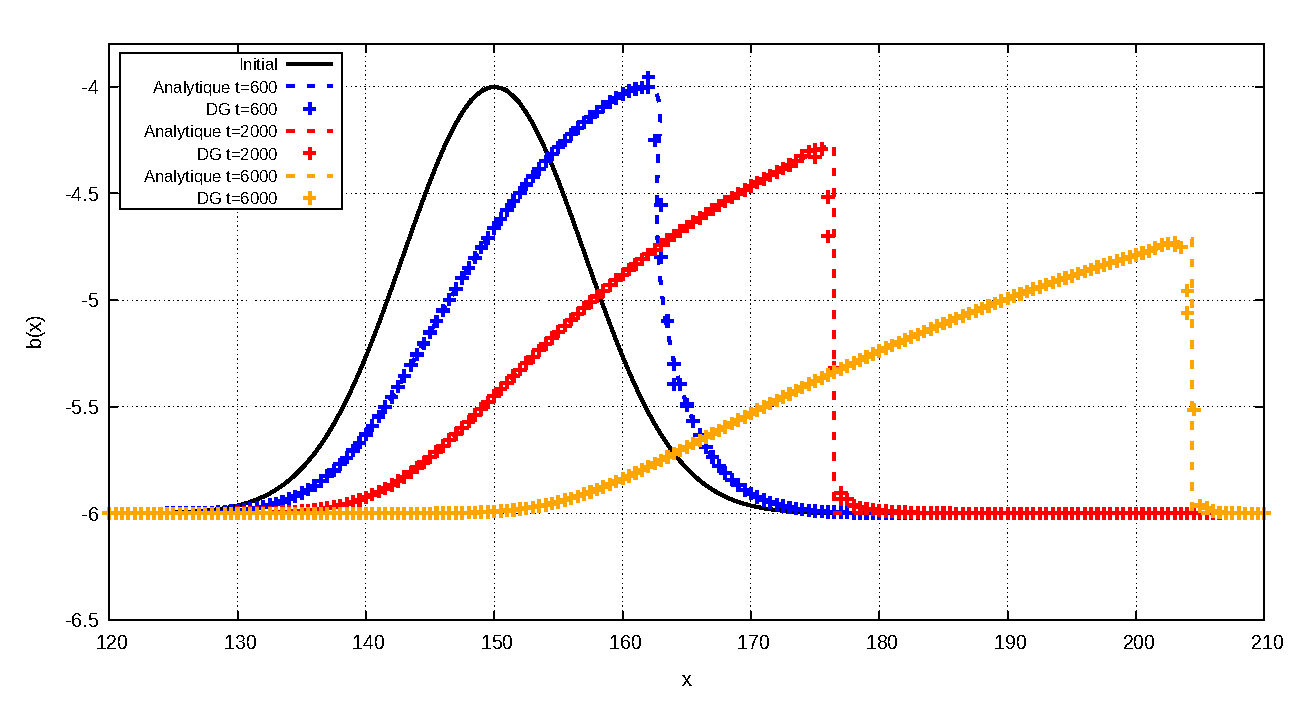
\includegraphics[width=0.96\linewidth]{PNG/Long/long_n_x_300_avec_limiteur.pdf}
    \caption{Cas test 2 -- Comparaison entre les solutions numériques (croix) avec limiteur de pente et la solution semi-analytique (traits) pour $p = 2$ et $N_x = 300$}
    \label{fig:impact_limiteur_long}
\end{figure}

D'un point de vue qualitatif, les solutions numériques approchent avec une grande précision la solution exacte dans les zones régulières. \\
Par ailleurs, cette comparaison permet de mettre en lumière deux caractéristiques fondamentales du schéma. D'une part, on observe graphiquement la signature structurelle des méthodes DG : à une même interface, la solution numérique peut posséder deux valeurs distinctes.
D'autre part, le limiteur de pente a tendance à diffuser le choc dans la mesure où nous voyons des points plus équitablement répartis à la discontinuité.

Enfin, concernant la conservation globale de la masse sédimentaire en double précision, on observe un écart de $6.65 \times 10^{-9}$ au temps final $t = \SI{6000}{\second}$. \\
Afin de vérifier la nature conservative du schéma, le calcul a été exécuté en quadruple précision. L'écart de masse chute alors à $8.30 \times 10^{-29}$, ce qui correspond au zéro machine pour ce niveau de précision après plusieurs milliers d'itérations. \\
Ce résultat suggère que le schéma est théoriquement conservatif. L'écart observé en double précision est ainsi \textit{a priori} dû à la propagation des erreurs d'arrondi numérique sur l'ensemble de la simulation.

\subsection{Cas test 3 : Solution semi-analytique de Fernandez-Nieto \textit{et al.}} \label{sec:Cas_test_2_4}

Ce dernier cas test s'inscrit dans une logique de pré-couplage avec les équations de Saint-Venant. \\
En s'appuyant sur les travaux de Fernandez-Nieto \textit{et al.} \cite{fernandez2025third}, une solution semi-analytique du système de Saint-Venant-Exner 1D peut être établie. \\
Cette dérivation repose sur l'hypothèse d'un flux sédimentaire $G$ régi par la loi de Grass, ainsi que sur une structure spécifique du triplet de conditions initiales $W_\text{ini} = (h_\text{ini}, u_\text{ini}, b_\text{ini})$, définie par
\begin{equation}
    h_\text{ini}(x) = h_0 \in \mathbb{P}^0, \quad u_\text{ini}(x) = A_{FN} x + B_{FN} \in \mathbb{P}^1, \quad b_\text{ini}(x) = \frac{3 \xi_0 A_G A_{FN}}{C_{FN}} u_\text{ini}^2(x) \in \mathbb{P}^2
\end{equation}
où $\xi_0 = 1/(1 - \varepsilon_0)$, $h_0 > 0$, $A_{FN}$, $B_{FN}$, $C_{FN}$ sont des constantes et l'exposant de Grass est fixé à $m_G = 3$. \\
Dès lors, si $\displaystyle \widetilde{W}(t) = \left( \widetilde{h}(t), \widetilde{u}(t), \widetilde{b}(t) \right)$ est une solution du problème
\begin{equation} \label{eq:Fernandez_Nieto_EDO}
    \left \{
    \begin{aligned}
        & \frac{\text{d}}{\text{d}t} \widetilde{h}(t) + A_{FN} \widetilde{u}(t) \widetilde{h}(t) = 0 \\
        & \frac{\text{d}}{\text{d}t} \widetilde{u}(t) + A_{FN} \widetilde{u}^2(t) + \frac{6 g \xi_0 A_G A_{FN}^2}{C_{FN}} \widetilde{b}(t) = 0 \\
        & \frac{\text{d}}{\text{d}t} \widetilde{b}(t) + C_{FN} \widetilde{u}^3(t) = 0 \\
        & \widetilde{\bm{W}}(0) = (h_0, 1, 1)
    \end{aligned}
    \right .
\end{equation}
alors
\begin{equation}
    \bm{W}(x, t) = \left( \widetilde{h}(t), u_\text{ini}(x) \widetilde{u}(t), b_\text{ini}(x) \widetilde{b}(t) \right)
\end{equation}
est une solution du système de Saint-Venant-Exner 1D muni d'une condition aux limites de Dirichlet à gauche, d'une condition aux limites de sortie libre à droite et de la condition initiale $\bm{W}(x, 0) = \bm{W}_\text{ini}(x)$. \\

Les cas tests 1 et 2 sont construits de sorte à faire intervenir une dépendance explicite en $b$ pour la vitesse $u$. \\
Cependant, dans le cas général, le flux $G$ ne dépend pas explicitement de $b$ (de sorte que $\partial_b G = 0$), ce qui est par exemple le cas de la loi de Grass. La dépendance par rapport au fond devient indirecte et dictée par la réponse de l'hydrodynamique. \\
Dans cette configuration, la vitesse de l'onde sédimentaire $\lambda_i^n$ ne peut plus être obtenue directement par la formule \eqref{eq:Vitesse_onde_sedimentaire}. Elle doit alors être exprimée à partir des valeurs propres de la Jacobienne associée à l'écriture sous forme vectorielle non conservative de \eqref{eq:Saint_Venant_Exner}. \\
Par linéarisation, on obtient la vitesse caractéristique locale de l'onde sédimentaire de De Vries, dont l'établissement en 2D sera détaillé dans le chapitre concernant le couplage avec les équations de Saint-Venant et dont la convergence vers la valeur propre 1D est présentée en annexe \ref{annexe:polynome_caracteristique}.
\begin{equation}
    \lambda_{i, \text{DV}}(x, t) = \frac{1}{m \left( \bm{\Phi}_i^T(x) \bm{\beta}_i(t) \right)} \left| \partial_q G \left( \bm{\Phi}_i^T(x) \bm{B}_i(t) \right) \frac{u(x, t)}{1 - \text{Fr}^2} \right|
\end{equation}
où $u(x, t) = u_\text{ini}(x) \widetilde{u}(t)$ et Fr est le nombre de Froude. \\
En outre, la stabilité globale du schéma nécessite également de prendre en compte les vitesses caractéristiques des ondes de Saint-Venant pour ce cas test. \\
On introduit ainsi la vitesse d'onde maximale
\begin{equation}
    \lambda_{i, \text{max}} = \max_{F \in \partial \Omega_i^n} \left( \max_{x \in F} \left( \left| u(x, t^n) - \sqrt{g h} \right|, \lambda_{i, \text{DV}}(x, t^n), \left| u(x, t^n) + \sqrt{g h} \right| \right) \right)
\end{equation}
Par conséquent, la condition CFL pour le pas de temps lié à l'advection est donnée par
\begin{equation}
    \max_{1 \leq i \leq N_x} \left( \frac{\lambda_{i, \text{max}}}{\Delta x_i} \right) \Delta t^A \leq \frac{1}{2 \max_i(p_i) + 1}
\end{equation}
Enfin, les constantes sont fixées conformément à l'article de Fernandez-Nieto \textit{et al.} afin d'avoir une comparaison qualitative des résultats. \\
Ainsi, on a les paramètres
\begin{equation}
    h_0 = 10, \quad A_{FN} = 0.01, \quad B_{FN} = 0.01, \quad C_{FN} = \xi_0 = 1, \quad A_G = 0.001
\end{equation}
De plus, par construction, la solution exacte pour la hauteur de la bathymétrie $b(x, t)$ est un polynôme de degré 2 en espace. En ce sens, utiliser un degré polynomial $p = 2$ pour l'espace DG n'aurait d'autre intérêt que de mesurer l'erreur intrinsèque de notre schéma. \\
Par conséquent, la figure \ref{fig:Comparaison_Fernandez_Nieto} ainsi que le tableau de convergence \ref{tab:convergence_fernandez_nieto} sont obtenus en fixant $p = 1$. \\

\begin{figure} [!t]
    \centering
    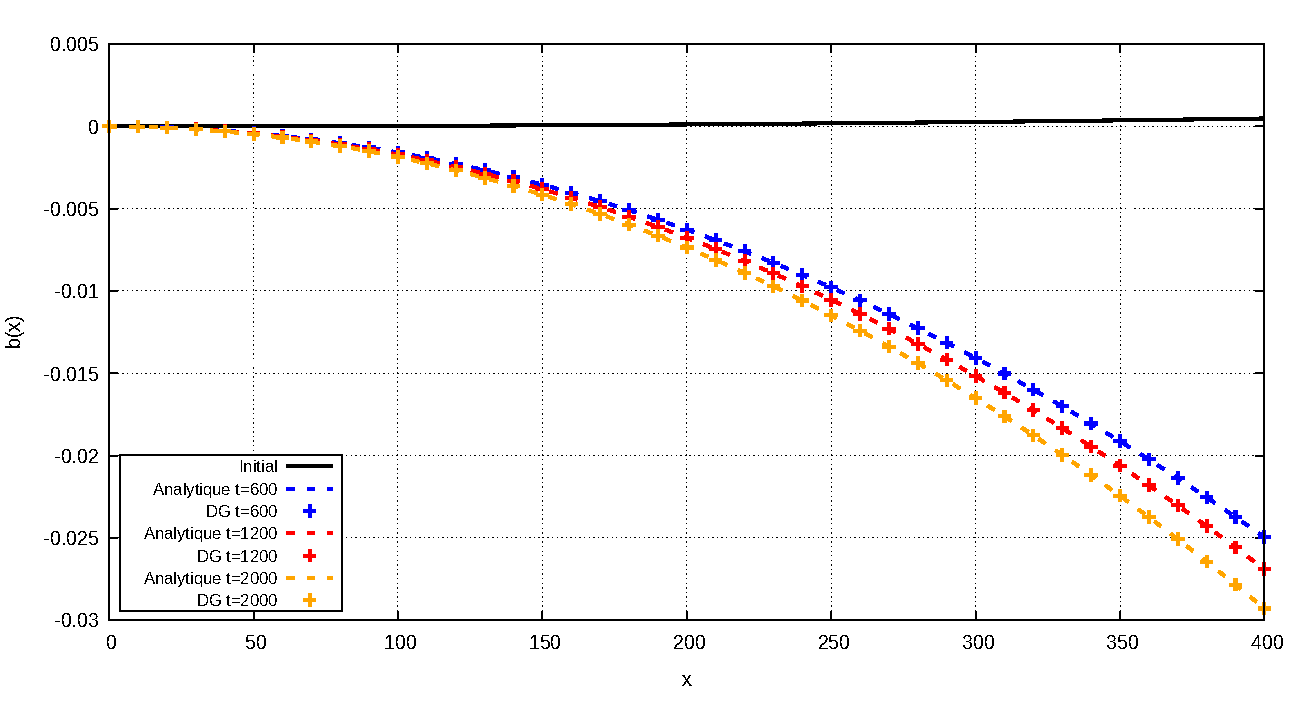
\includegraphics[width=0.96\linewidth]{PNG/Fernandez_Nieto/fernandez_nieto_n_x_40.pdf}
    \caption{Cas test 3 -- Comparaison entre la solution numérique (croix) et la solution semi-analytique (traits) à différents instants pour $p = 1$ et $N_x = 40$}
    \label{fig:Comparaison_Fernandez_Nieto}
\end{figure}

Qualitativement, la solution numérique concorde avec la solution semi-analytique, validant ainsi notre implémentation vis-à-vis de \cite{fernandez2025third}. Sur le plan quantitatif, les erreurs en normes $L^2$ et $L^\infty$, ainsi que l'ordre de convergence associé, sont rassemblés dans le tableau \ref{tab:convergence_fernandez_nieto}. On y retrouve bien l'ordre théorique optimal du schéma DG, i.e. $p+1 = 2$.

\begin{table}[H]
    \centering
    \small
    \begin{tabular}{r ccc}
    \toprule
    $N_x$ & $L^2$ & $L^\infty$ & Ordre \\
    \midrule
    10 & 4.34E-04 & 2.97E-05 & -- \\
    20 & 1.08E-04 & 7.34E-06 & 2.00 \\
    40 & 2.71E-05 & 1.85E-06 & 1.99 \\
    80 & 6.79E-06 & 4.64E-07 & 1.99 \\
    \bottomrule
    \end{tabular}
    \caption{Cas test 3 -- Erreurs d'approximation en norme $L^2$, $L^\infty$ au temps $t = \SI{2000}{\second}$ et ordres de convergence associés pour $p = 1$}
    \label{tab:convergence_fernandez_nieto}
\end{table}

\chapter{Système d'équations de Saint-Venant-Exner et formulation de Galerkin discontinue}

Ce chapitre établit l'analyse spectrale 2D du système couplé Saint-Venant-Exner \eqref{eq:Saint_Venant_Exner}, dérive la valeur propre de De Vries 2D, puis formule le schéma RKDG complet.
Nous nous intéressons alors au système d'équations
\begin{equation} \tag{$\mathcal{SWE}$} \label{eq:Saint_Venant_Exner}
    \left \{
    \begin{aligned}
        & \partial_t h + \nabla \cdot \left( h \bm{u} \right) = 0 && \text{sur } \Omega \times (0, T) \\
        & \partial_t (h \bm{u}) + \nabla \cdot \left( h \bm{u} \otimes \bm{u} + g \frac{h^2}{2} \mathbb{I} \right) = - g h \nabla b && \text{sur } \Omega \times (0, T) \\
        & m(\nabla b) \partial_t b + \nabla \cdot \bm{G} = S && \text{sur } \Omega \times (0, T) \\
        & + \text{Conditions aux limites} \\
        & + \text{Conditions initiales}
    \end{aligned}
    \right .
\end{equation}

L'étude des valeurs propres de \eqref{eq:Saint_Venant_Exner} est primordiale car, d'une part, elles permettent de déterminer le domaine d'hyperbolicité du système et, d'autre part, elles sont utilisées pour définir la diffusion numérique des flux de Rusanov. \\
Ainsi, en introduisant le débit hydraulique $\bm{q} = (q_x, q_y) = h \bm{u} = (hu, hv)$, le système de Saint-Venant-Exner sous forme quasi-conservative s'écrit :
\begin{equation}
    \left \{
    \begin{aligned}
        & \partial_t h + \partial_x q_x + \partial_y q_y = 0 \\
        & \partial_t q_x + \partial_x \left( \frac{q_x^2}{h} + g \frac{h^2}{2} \right) + \partial_y \left( \frac{q_x q_y}{h} \right) = - g h \partial_x b \\
        & \partial_t q_y + \partial_x \left( \frac{q_x q_y}{h} \right) + \partial_y \left( \frac{q_y^2}{h} + g \frac{h^2}{2} \right) = - g h \partial_y b \\
        & m(\nabla b) \partial_t b + \partial_x G_x + \partial_y G_y = S
    \end{aligned}
    \right .
\end{equation}
où $G_x$ et $G_y$ sont les composantes suivant $x$ et $y$ du flux sédimentaire $\bm{G}$. \\
Ce système d'équations peut se réécrire sous la forme matricielle
\begin{equation}
    \mathbb{M}(\nabla b) \partial_t \bm{W} + \nabla \cdot \mathbb{G}(\bm{W}) = \bm{S}(\bm{W})
\end{equation}
où $\bm{W} = (h, q_x, q_y, b)^T$ désigne le vecteur des variables d'état, $\mathbb{M}(\nabla b) = \text{diag}(1, 1, 1, m(\nabla b))$ est la matrice liée à la métrique géométrique et $\mathbb{G}(\bm{W}) = (\bm{G}_1(\bm{W}), \bm{G}_2(\bm{W}))$ est le tenseur des flux physiques conservatifs avec
\begin{equation}
    \bm{G}_1(\bm{W}) = \begin{pmatrix}
        q_x \\
        \frac{q_x^2}{h} + g \frac{h^2}{2} \\
        \frac{q_x q_y}{h} \\
        G_x
    \end{pmatrix}, \quad
    \bm{G}_2(\bm{W}) = \begin{pmatrix}
        q_y \\
        \frac{q_y^2}{h} + g \frac{h^2}{2} \\
        \frac{q_y q_x}{h} \\
        G_y
    \end{pmatrix}, \quad
    \bm{S}(\bm{W}) = \begin{pmatrix}
        0 \\
        - gh \partial_x b \\
        - gh \partial_y b \\
        S
    \end{pmatrix}
\end{equation}
Afin de pouvoir mener l'étude spectrale, il est nécessaire de passer à la forme quasi-linéaire
\begin{equation}
    \partial_t \bm{W} + \mathbb{J}_1(\bm{W}) \partial_x \bm{W} + \mathbb{J}_2(\bm{W}) \partial_y \bm{W} = \bm{S}_\text{ext}(\bm{W})
\end{equation}
avec $\bm{S}_\text{ext}(\bm{W}) = (0, 0, 0, S/m(\nabla b))^T$ le vecteur de termes sources externes (lié aux caractéristiques du lit sédimentaire) et
\begin{equation}
    \begin{aligned}
        \mathbb{J}_1(\bm{W}) & = \mathbb{M}^{-1}(\nabla b) \frac{\partial \bm{G}_1(\bm{W})}{\partial \bm{W}} + \begin{pmatrix}
            0 & 0 & 0 & 0 \\
            0 & 0 & 0 & gh \\
            0 & 0 & 0 & 0 \\
            0 & 0 & 0 & 0 \\
        \end{pmatrix}
        = \begin{pmatrix}
            0 & 1 & 0 & 0 \\
            gh - u^2 & 2u & 0 & gh \\
            -uv & v & u & 0 \\
            \alpha_x & \beta_x & \gamma_x & 0
        \end{pmatrix} \\
        \mathbb{J}_2(\bm{W}) & = \mathbb{M}^{-1}(\nabla b) \frac{\partial \bm{G}_2(\bm{W})}{\partial \bm{W}} + \begin{pmatrix}
            0 & 0 & 0 & 0 \\
            0 & 0 & 0 & 0 \\
            0 & 0 & 0 & gh \\
            0 & 0 & 0 & 0 \\
        \end{pmatrix}
        = \begin{pmatrix}
            0 & 0 & 1 & 0 \\
            - uv & v & u & 0 \\
            gh - v^2 & 0 & 2v & gh \\
            \alpha_y & \beta_y & \gamma_y & 0
        \end{pmatrix}
    \end{aligned}
\end{equation}
où, similairement pour $x$ et $y$,
\begin{equation}
    \alpha_x = \frac{1}{m(\nabla b)} \frac{\partial G_x}{\partial h}, \quad \beta_x = \frac{1}{m(\nabla b)} \frac{\partial G_x}{\partial q_x}, \quad \gamma_x = \frac{1}{m(\nabla b)} \frac{\partial G_x}{\partial q_y}
\end{equation}
Pour que le système \eqref{eq:Saint_Venant_Exner} soit strictement hyperbolique, il est nécessaire que les valeurs propres de
\begin{equation}
    \mathbb{H}(\bm{W}) = \mathbb{J}_1 n_x + \mathbb{J}_2 n_y = \begin{pmatrix}
        0 & n_x & n_y & 0 \\
        (gh - u^2) n_x - uv n_y & 2u n_x + v n_y & u n_y & gh n_x \\
        (gh - v^2) n_y - uv n_x & v n_x & 2v n_y + u n_x & gh n_y \\
        \alpha_n & \beta_n & \gamma_n & 0
    \end{pmatrix}
\end{equation}
soient réelles et distinctes selon toute direction $\bm{n} = (n_x, n_y)$ avec $\bm{n}$ une normale unitaire et
\begin{equation}
    \alpha_n = \alpha_x n_x + \alpha_y n_y, \quad \beta_n = \beta_x n_x + \beta_y n_y, \quad \gamma_n = \gamma_x n_x + \gamma_y n_y
\end{equation}
Le développement en Annexe \ref{annexe:polynome_caracteristique} nous conduit au polynôme caractéristique de $\mathbb{H}$ suivant :
\begin{equation} \label{eq:Polynome_caracteristique}
    \chi_H = \lambda(\lambda - u_n) \left[ (\lambda - u_n)^2 - gh \right] - gh \left[ \delta_n \lambda^2 + \left( \alpha_n - u_n \delta_n + u_t \delta_t \right) \lambda - u_n \left( \alpha_n + u_t \delta_t \right) \right]
\end{equation}
où nous avons posé $u_n = u n_x + v n_y$ et $u_t = u n_y - v n_x$ les composantes normale et tangentielle de la vitesse, $\delta_n = \beta_n n_x + \gamma_n n_y$ et $\delta_t = \beta_n n_y - \gamma_n n_x$ les sensibilités du flux sédimentaire aux variations de débit normal et tangentiel respectivement.

Cette dernière écriture met en avant l'impact de l'équation d'Exner sur les valeurs propres usuelles du système de Saint-Venant. \\
En effet, si nous considérons un fond fixe, alors $\alpha_n = \delta_n = \delta_t = 0$ donc :
\begin{equation}
    \chi_H(\lambda) = \lambda(\lambda - u_n) \left[ (\lambda - u_n)^2 - gh \right] = \lambda (\lambda - u_n) \left( \lambda - \left[u_n - \sqrt{gh}\right] \right) \left( \lambda - \left[ u_n + \sqrt{gh} \right] \right)
\end{equation}
Nous reconnaissons ainsi les trois valeurs propres usuelles de Saint-Venant, ainsi qu'une quatrième valeur propre nulle liée à la bathymétrie fixe. \\
Par conséquent, l'équation d'Exner agit comme une perturbation de la vitesse des ondes du système de Saint-Venant.

\begin{samepage}
De plus, le polynôme caractéristique \eqref{eq:Polynome_caracteristique} nous permet de retrouver la valeur propre de De Vries en 1D et d'étendre cette dernière en 2D. \\
Pour ce faire, comme l'échelle de temps de l'évolution de la bathymétrie est lente devant la dynamique de l'eau en régime sous-critique, l'idée de De Vries \cite{vries1965considerations} est d'effectuer un développement limité à l'ordre 1 autour de $\lambda = 0$.
Ainsi, il vient
\begin{equation}
    - \left[ u_n(u_n^2 - gh) + gh \left( \alpha_n - u_n \delta_n + u_t \delta_t \right) \right] \lambda_\text{DV} + gh u_n \left[ \alpha_n + u_t \delta_t \right] = 0
\end{equation}
soit
\begin{equation}
    \lambda_\text{DV} = \frac{\left( \alpha_n + u_t \delta_t \right) u_n}{-u_n \left( 1 - \text{Fr}_n^2 \right) + \alpha_n + u_t \delta_t - u_n \delta_n}
\end{equation}
\end{samepage}

\section{Formulation semi-discrète et discrète}

La résolution numérique s'appuie sur un couplage faible scindé en deux sous-problèmes $(\mathcal{SW})$ et \eqref{eq:Exner_generalisee}. À chaque sous-pas de temps du schéma temporel, chaque sous-système est résolu séquentiellement en gelant le vecteur d'état de l'autre. Nous assemblons ainsi la formulation RKDG \textit{well-balanced} de Saint-Venant développée par Camille Poussel dans sa thèse \cite{poussel2024dynamique} et celle d'Exner développée dans ce travail.
Le problème matriciel semi-discret pour le système \eqref{eq:Saint_Venant_Exner} s'écrit
\begin{equation} \tag{$\mathcal{P}_M^\mathcal{SWE}$}
    \left \{
    \begin{aligned}
        & \forall i \in \llbracket 1, N_e \rrbracket, \text{ trouver } \bm{W}_i = (h_i, \bm{q}_i) \in \mathbb{R}^{3N_\text{ddl}^i} \text{ et } \bm{B}_i \in \mathbb{R}^{N_\text{ddl}^i} \text{ tels que} \\
        & \mathbb{M}_i^\mathcal{SW} \partial_t \bm{W}_i(t) = \bm{\mathcal{I}}_i^{\mathcal{SW}, EF} \left( \bm{W}_i \right) - \bm{\mathcal{I}}_i^{\mathcal{SW}, VF} \left( \bm{W}_i, \bm{B}_i \right) + \bm{\mathcal{I}}_i^{\mathcal{SW}, S} \left( \bm{W}_i, \bm{B}_i \right) \\
        & \mathbb{M}_i^\mathcal{E}(t) \partial_t \bm{B}_i(t) = \bm{\mathcal{I}}_i^{\mathcal{E}, EF} \left( \bm{B}_i, \bm{W}_i , \tau_i \right) - \bm{\mathcal{I}}_i^{\mathcal{E}, VF} \left( \bm{B}, \bm{W}, \bm{\tau} \right) + \bm{\mathcal{I}}_i^{\mathcal{E}, S} \left( \bm{B}_i, \bm{W}_i, \tau_i \right) \\
        & \bm{W}_i(0) = \bm{W}_i^0 \\
        & \bm{B}_i(0) = \bm{B}_i^0
    \end{aligned}
    \right .
\end{equation}
où les annotations $\mathcal{SW}$ et $\mathcal{E}$ font référence aux intégrales définies dans les problèmes matriciels de Saint-Venant et d'Exner respectivement. \\

En suivant la même démarche que pour l'équation d'Exner, nous introduisons $\bm{L}_i^\mathcal{SW}$ et $\bm{L}_i^\mathcal{E}$ les composantes $i$ des opérateurs issus de la méthode des lignes pour les équations $(\mathcal{SW})$ et \eqref{eq:Exner_generalisee}. \\
Ainsi, nous pouvons écrire que
\begin{equation}
    \begin{aligned}
        & \partial_t \bm{W}_i(t) = \bm{L}_i^{\mathcal{SW}, E} \left( \bm{W}_i, \bm{B}_i \right) \\
        & \partial_t \bm{B}_i(t) = \bm{L}_i^{\mathcal{E}, E} \left( \bm{B}, \bm{W}, \bm{\tau} \right) + \bm{L}_i^{\mathcal{E}, I} \left( \bm{B}_i, \bm{W}_i, \tau_i \right)
    \end{aligned}
\end{equation}
où les exposants $E$ et $I$ font référence à des opérateurs explicites et implicites respectivement. \\
En particulier, ils s'expriment comme
\begin{equation}
    \begin{aligned}
        \bm{L}_i^{\mathcal{SW}, E} \left( \bm{W}_i, \bm{B}_i \right) & = \left( \mathbb{M}_i^\mathcal{SW} \right)^{-1} \left[ \bm{\mathcal{I}}_i^{\mathcal{SW}, EF} \left( \bm{W}_i \right) - \bm{\mathcal{I}}_i^{\mathcal{SW}, VF} \left( \bm{W}_i, \bm{B}_i \right) + \bm{\mathcal{I}}_i^{\mathcal{SW}, S} \left( \bm{W}_i, \bm{B}_i \right) \right] \\
        \bm{L}_i^{\mathcal{E}, E} \left( \bm{B}, \bm{W}, \bm{\tau} \right) & = \left( \mathbb{M}_i^\mathcal{E}(t) \right)^{-1} \left[ \bm{\mathcal{I}}_i^{\mathcal{E}, EF} \left( \bm{B}_i, \bm{W}_i, \tau_i \right) - \bm{\mathcal{I}}_i^{\mathcal{E}, VF} \left( \bm{B}, \bm{W}, \bm{\tau} \right) \right] \\
        \bm{L}_i^{\mathcal{E}, I} \left( \bm{B}_i, \bm{W}_i, \tau_i \right) & = \left( \mathbb{M}_i^\mathcal{E}(t) \right)^{-1} \bm{\mathcal{I}}_i^{\mathcal{E}, S} \left( \bm{B}_i, \bm{W}_i , \tau_i \right)
    \end{aligned}
\end{equation}
avec $\bm{W} \in \mathbb{R}^{3N_\text{ddl}}$ le vecteur contenant les $N_e$ vecteurs d'états issus des équations de Saint-Venant et $\bm{B} \in \mathbb{R}^{N_\text{ddl}}$ le vecteur contenant les $N_e$ vecteurs de bathymétrie $\bm{B}_i$. \\
En ce sens, pour une étape $s \leq m$, la formulation discrète RKDG des équations de Saint-Venant-Exner s'écrit
\begin{equation}
    \begin{aligned}
        & \bm{W}_i^{(s)} = \bm{W}_i^n + \Delta t^n \sum_{j = 1}^{s-1} \widetilde{a}_{s, j} \bm{L}_i^{\mathcal{SW}, E} \left( \bm{W}_i^{(j)}, \bm{B}_i^{(j)} \right) \\
        & \bm{B}_i^{(s)} - \Delta t^n a_{s, s} \bm{L}_i^{\mathcal{E}, I} \left( \bm{B}_i^{(s)}, \bm{W}_i^{(s)}, \tau_i^{(s)} \right) = \bm{B}_i^n + \Delta t^n \sum_{j = 1}^{s-1} \widetilde{a}_{s, j} \bm{L}_i^{\mathcal{E}, E} \left( \bm{B}^{(j)}, \bm{W}^{(j)}, \bm{\tau}^{(j)} \right) \\
        & \phantom{\bm{B}_i^{(s)} - \Delta t^n a_{s, s} \bm{L}_i^{\mathcal{E}, I} \left( \bm{B}_i^{(s)}, \bm{W}_i^{(s)}, \tau_i^{(s)} \right) = \bm{B}_i^n } + \Delta t^n \sum_{j = 1}^{s-1} a_{s, j} \bm{L}_i^{\mathcal{E}, I} \left( \bm{B}_i^{(j)}, \bm{W}_i^{(j)}, \tau_i^{(j)} \right)
    \end{aligned}
\end{equation}
Une fois les $m$ stages évalués, les vecteurs d'états au temps $t^{n+1}$ s'expriment
\begin{equation} \tag{$\mathcal{P}_D^\mathcal{SWE}$} \label{eq:Probleme_discret_Saint_Venant_Exner}
    \begin{aligned}
        & \bm{W}_i^{n+1} = \bm{W}_i^n + \Delta t^n \sum_{j = 1}^{m} \widetilde{b}_j \bm{L}_i^{\mathcal{SW}, E} \left( \bm{W}_i^{(j)}, \bm{B}_i^{(j)} \right) \\
        & \bm{B}_i^{n+1} = \bm{B}_i^n + \Delta t^n \sum_{j = 1}^{m} \widetilde{b}_j \bm{L}_i^{\mathcal{E}, E} \left( \bm{B}^{(j)}, \bm{W}^{(j)}, \bm{\tau}^{(j)} \right) + \Delta t^n \sum_{j = 1}^{m} b_j \bm{L}_i^{\mathcal{E}, I} \left( \bm{B}_i^{(j)}, \bm{W}_i^{(j)}, \tau_i^{(j)} \right)
    \end{aligned}
\end{equation}

Enfin, comme une partie du schéma temporel est explicite, nous sommes soumis à une condition CFL. Sur la base des travaux de Cockburn et Shu \cite{cockburn2001runge}, cette dernière peut être estimée par
\begin{equation}
    \max_{i \in \llbracket 1, N_e \rrbracket} \left( \frac{\lambda_i^n}{d_i} \right) \Delta t^A \leq \frac{1}{2 \max_i(p_i) + 1}
\end{equation}
avec $d_i$ le diamètre de la maille $\Omega_i^n$ et $\lambda_i^n$ la plus grande vitesse caractéristique des ondes sur la maille, i.e.
\begin{equation}
    \lambda_i^n = \max_{F \in \partial \Omega_i^n} \left( \max_{\bm{x} \in F} \left( \left| \bm{u}(\bm{x}, t^n) \cdot \bm{n}_F - \sqrt{gh} \right|, \left| \lambda_\text{DV} (\bm{x}, t^n) \right|, \left| \bm{u}(\bm{x}, t^n) \cdot \bm{n}_F + \sqrt{gh} \right| \right) \right)
\end{equation}
Pour finir, on multiplie le pas de temps par un facteur de sûreté $\alpha_\text{CFL} \in (0,1)$, de telle sorte que
\begin{equation}
    \Delta t^n = \alpha_\text{CFL} \Delta t^A
\end{equation}

\chapter*{Conclusion et perspectives}
\addcontentsline{toc}{chapter}{Conclusion et perspectives}

Ce travail de stage s'est consacré à la résolution numérique de l'équation d'Exner généralisée en formulations 1D et 2D. L'approche développée repose sur des méthodes \textit{Runge-Kutta Discontinuous Galerkin}, adaptées pour atteindre un ordre élevé d'approximation spatio-temporelle tout en assurant une capture précise des chocs et des raideurs. L'évaluation de plusieurs schémas temporels a conduit au choix d'un schéma \textit{Implicit-Explicit}, offrant un compromis idéal entre stabilité et efficacité numérique face au terme source. \\
Les solveurs 1D et 2D développés ont été validés avec succès à l'aide d'une solution manufacturée et de cas tests de référence issus de la littérature (Long \textit{et al.}, Fernandez-Nieto \textit{et al.}). Ces configurations ont permis de vérifier l'obtention de l'ordre de convergence théorique $p+1$, de démontrer la robustesse du schéma en présence de fortes raideurs, et d'initier un premier cadre de pré-couplage avec le modèle hydrodynamique de Saint-Venant. \\
Enfin, le dernier chapitre a posé les fondements théoriques et la discrétisation RKDG complète du système couplé Saint-Venant-Exner. \\

Les résultats et le cadre formel établis au cours de ce travail ouvrent des perspectives d'extension particulièrement prometteuses :
\begin{itemize}
    \item \textbf{Implémentation du schéma RKDG couplé dans RIVAGE :} L'étape immédiate consiste à finaliser l'intégration numérique du schéma RKDG pour le système complet de Saint-Venant-Exner au sein du code de calcul RIVAGE.
    \item \textbf{Préservation des équilibres :} Une attention particulière devra être portée à la construction d'un schéma préservant exactement les états d'équilibre hydrostatiques en présence de l'équation d'Exner (pour l'instant la propriété de \textit{well-balancedness} n'est développée que pour les équations de Saint-Venant).
    \item \textbf{Validation sur cas tests expérimentaux :} Il s'agira d'évaluer le comportement du code sur des cas complexes de type rupture de barrage sur bathymétrie érodable, en comparant notamment les performances des différentes lois empiriques de charriage (Grass, MPM, Van Rijn).
    \item \textbf{Extension au couplage avec le milieu poreux :} Enfin, le couplage avec le modèle de Richards pour prendre en compte les processus d'infiltration/exfiltration permettrait d'aboutir à un système triplement couplé Saint-Venant-Exner-Richards, ouvrant la voie à une modélisation globale des interactions surface-sous-sol en zone côtière.
\end{itemize}

\begin{appendices}

% Personnalisation pour le français
\renewcommand{\appendixtocname}{Annexes}
\renewcommand{\chaptername}{Annexe}

% Compteurs d'équations, figures et tableaux (A.1, A.2, etc.)
\counterwithin{equation}{chapter}
\counterwithin{figure}{chapter}
\counterwithin{table}{chapter}

\chapter{Présentation de la méthode de Galerkin discontinue sur l'équation de transport en 1D}
\label{annexe:DG_1D}

Cette annexe établit la formulation matricielle semi-discrète DG de l'équation de transport en 1D et met en évidence les liens entre le schéma DG et les schémas EF et VF usuels. \\

On s'intéresse à la résolution du problème : trouver $u(x, t) : \Omega \times (0, T) \longrightarrow \mathbb{R}$ tel que
\begin{equation} \tag{$\mathcal{T}$} \label{eq:Transport_forte}
    \left \{
    \begin{aligned}
        &\partial_t u(x, t) + \partial_x G(u) = 0   &&\text{sur } \Omega \times (0, T) \\
        &u(x, t) = u_D(x, t)                        &&\text{sur } \Gamma_D \times (0, T) \\
        &G(u(x,t)) \cdot n = q_N(x, t)              &&\text{sur } \Gamma_N \times (0, T) \\
        &u(x, 0) = u_\text{ini}(x)                  &&\text{sur } \Omega
    \end{aligned}
    \right .
\end{equation}
avec $G(u) = au$, $a \in \mathbb{R}$ fixé, où $\Gamma_D$ et $\Gamma_N$ désignent les frontières de Dirichlet et de Neumann. \\

La formulation variationnelle semi-discrète DG s'obtient de manière en tout point semblable à une méthode EF : on multiplie l'équation de transport par une fonction test $\varphi \in \mathcal{V}^{\mathbf{p}}(\mathcal{M})$ puis on intègre sur l'ensemble des mailles $\Omega_i$ du maillage $\mathcal{M}$, ce qui donne le problème
\begin{equation} \tag{$\mathcal{P}_{SD}^\mathcal{T}$} \label{eq:Probleme_variationnel_transport}
    \left \{
    \begin{aligned}
        &\text{Trouver } u_h \in \mathcal{V}^{\mathbf{p}}(\mathcal{M}) \text{ tel que } \forall \varphi \in \mathcal{V}^{\mathbf{p}}(\mathcal{M}) \\
        &m_\mathcal{T}(\partial_t u_h, \varphi) + a_\mathcal{T}(u_h, \varphi) = l_\mathcal{T}(\varphi) 
    \end{aligned}
    \right .
\end{equation}
où les formes bilinéaires DG $m_\mathcal{T}$ et $a_\mathcal{T}$, et la forme linéaire $l_\mathcal{T}$ sont définies comme
\begin{equation}
    \begin{aligned}
        \forall v, \varphi \in \mathcal{V}^{\mathbf{p}}(\mathcal{M}), ~ & m_\mathcal{T}(v, \varphi) = \sum_{\Omega_i \in \mathcal{M}} \int_{\Omega_i} v \varphi \text{d}x \\
        & a_\mathcal{T}(v, \varphi) = - \sum_{\Omega_i \in \mathcal{M}} \int_{\Omega_i} G(v) \partial_x \varphi \text{d}x - \sum_{F \in \mathcal{F}^\text{int}} \int_F \widehat{G}_F(v) \llbracket \varphi \rrbracket \text{d}F \\
        & l_\mathcal{T}(\varphi) = - \sum_{F \in \mathcal{F}_D^\partial} \int_F (a u_D \cdot n_F) \varphi \text{d}F - \sum_{F \in \mathcal{F}_N^\partial} \int_F q_N \varphi \text{d}F
    \end{aligned}
\end{equation}
avec $\mathcal{F}^\text{int}$ l'ensemble des interfaces des mailles intérieures de $\mathcal{M}$, $\mathcal{F}_D^\partial$ et $\mathcal{F}_N^\partial$ sont les interfaces de $\mathcal{M}$ soumises à des conditions aux limites de Dirichlet et Neumann respectivement, $\widehat{G}_F$ est un flux numérique de G à l'interface $F$, $n_F$ est la normale unitaire de $F$ pointant de $\Omega_i$ vers la maille adjacente par l'interface $F$ ou vers l'extérieur du domaine pour une interface de bord, et on a introduit
\begin{equation}
    \forall F \in \mathcal{F}^\text{int}, \forall x \in F, ~ \llbracket v \rrbracket(x) = v_r(x) - v_l (x)
\end{equation}
le saut de $v$ à l'interface $F$. \\

La formulation \eqref{eq:Probleme_variationnel_transport} met en évidence la double nature de la méthode DG évoquée au début de cette partie. \\
D'une part, si la fonction test $\varphi$ est continue, alors $\llbracket \varphi \rrbracket = 0$ et on retrouve la formulation variationnelle semi-discrète EF. \\
D'autre part, si le degré de l'espace DG $p$ est fixé à 0, alors $\varphi$ est constante par morceaux, donc $\partial_x \varphi = 0$. Plus précisément, $\varphi = \mathds{1}_{\Omega_i}$, donc $\llbracket \varphi \rrbracket(x_{i - \sfrac{1}{2}}) = 1$ et $\llbracket \varphi \rrbracket(x_{i + \sfrac{1}{2}}) = -1$. On obtient alors les flux numériques $\widehat{G}_{i + \sfrac{1}{2}}$ et $\widehat{G}_{i - \sfrac{1}{2}}$ du schéma VF. \\
\begin{samepage}
    En effet, si $\partial \Omega_i$ est l'ensemble des faces de la maille $\Omega_i$, alors
    \begin{equation}
        \sum_{F \in \mathcal{F}^\text{int}} \int_F \widehat{G}_F(u) \llbracket \varphi \rrbracket \text{d}F = - \sum_{\Omega_i \in \mathcal{M}} \sum_{F \in \partial \Omega_i \cap \mathcal{F}^\text{int}} \int_F (\widehat{G}_F(u) \cdot n_F) \varphi \text{d}F
    \end{equation}
    car $\restricdynamic{\varphi}{\Omega_i} = 1$, $n_F(x_{i-\sfrac{1}{2}}) = -1$ et $n_F(x_{i+\sfrac{1}{2}}) = 1$.
\end{samepage}

Ainsi, en $p = 0$, le problème variationnel semi-discret \eqref{eq:Probleme_variationnel_transport} s'écrit
\begin{equation}
    \left \{
    \begin{aligned}
        &\text{Trouver } u_h \in \mathcal{V}^0(\mathcal{M}) \text{ tel que} \\
        &\sum_{\Omega_i \in \mathcal{M}} \int_{\Omega_i} \partial_t u_h \text{d}x + \sum_{\Omega_i \in \mathcal{M}} \sum_{F \in \partial \Omega_i \cap \mathcal{F}^\text{int}} \int_F \widehat{G}_F(u) \cdot n_F \text{d}F \\
        &+ \sum_{F \in \mathcal{F}_D^\partial} \int_F a u_D \cdot n_F \text{d}F + \sum_{F \in \mathcal{F}_N^\partial} \int_F q_N \text{d}F = 0
    \end{aligned}
    \right .
\end{equation}
ce qui correspond à la formulation semi-discrète VF de l'équation \eqref{eq:Transport_forte}. \\
Enfin, en pratique, les flux numériques sont choisis de sorte à obtenir un schéma VF (et par extension DG) stable comme le flux \textit{upwind} pour le problème de transport et le flux de Rusanov (ou de Lax-Friedrich local) pour les équations \eqref{eq:Exner_generalisee} et \eqref{eq:Saint_Venant_Exner}. \\

Grâce aux notations que l'on a introduites dans l'équation \eqref{eq:Projection_DG}, le problème variationnel \eqref{eq:Probleme_variationnel_transport} peut s'écrire sous la forme matricielle locale
\begin{equation} \tag{$\mathcal{P}_M^\mathcal{T}$} \label{eq:Probleme_matriciel_transport}
    \left \{
    \begin{aligned}
        & \forall i \in \llbracket 1, N_x \rrbracket, \text{ trouver } \bm{U}_{i} \in \mathbb{R}^{p_i + 1} \text{ tel que} \\
        &\mathbb{M}_i \partial_t \bm{U}_i(t) = \bm{\mathcal{I}}_i^{EF}(t) - \bm{\mathcal{I}}_i^{VF}(t) \\
        &\bm{U}_i(0) = \bm{U}_i^0
    \end{aligned}
    \right .
\end{equation}
avec
\begin{itemize}
    \item $\displaystyle \mathbb{M}_i = \int_{\widehat{\Omega}} \bm{\Phi}_i (\widehat{\phi}_i(\xi)) \bm{\Phi}_i^T(\widehat{\phi}_i(\xi)) \frac{\Delta x_i}{2} \text{d}\xi \in \mathbb{R}^{(p_i+1) \times (p_i+1)}$ la matrice de masse
    \item $\displaystyle \bm{\mathcal{I}}_i^{EF}(t) = \int_{\widehat{\Omega}} \frac{2}{\Delta x_i} \partial_\xi \bm{\Phi}_i(\widehat{\phi}_i(\xi)) G \left( \bm{\Phi}_i^T(\widehat{\phi}_i(\xi)) \bm{U}_i(t) \right) \frac{\Delta x_i}{2} \text{d}\xi \in \mathbb{R}^{p_i+1}$ le vecteur de contribution volumique du flux
    \item $\displaystyle \bm{\mathcal{I}}_i^{VF}(t) = \widehat{G}_{i + \sfrac{1}{2}} \bm{\Phi}_i(\widehat{\phi}_i(1)) - \widehat{G}_{i-\sfrac{1}{2}} \bm{\Phi}_i(\widehat{\phi}_i(-1)) \in \mathbb{R}^{p_i+1}$ le vecteur de contribution du flux aux interfaces
\end{itemize}
Afin d'alléger les notations, on sous-entendra désormais que
\begin{equation}
    \bm{\Phi}_i(\xi) = \bm{\Phi}_i(\widehat{\phi}_i(\xi)), \quad \mathbb{D}_i(\xi) = \mathbb{D}_i(\widehat{\phi}_i(\xi))
\end{equation}
Pour obtenir la formulation semi-discrète matricielle locale \eqref{eq:Probleme_matriciel_transport}, on exprime $u_h$ et $\varphi$ suivant la relation établie en \eqref{eq:Projection_DG}, ce qui donne
\begin{equation}
    \varphi(x) = \bm{V}^T \bm{\Phi}(x) \quad \text{et} \quad u_h(x, t) = \bm{\Phi}^T(x) \bm{U}(t)
\end{equation}
Ainsi, on a que
\begin{equation}
    \begin{aligned}
        &m_\mathcal{T}(\partial_t u_h, \varphi) = \sum_{\Omega_i \in \mathcal{M}} \int_{\Omega_i} \varphi \partial_t u_h \text{d}x \\
        &\phantom{m_\mathcal{T}(\partial_t u_h, \varphi) } = \sum_{\Omega_i \in \mathcal{M}} \int_{\Omega_i} \bm{V}^T \bm{\Phi}(x) \bm{\Phi}^T(x) \partial_t \bm{U}(t) \text{d}x \\
        &\phantom{m_\mathcal{T}(\partial_t u_h, \varphi) } = \sum_{\Omega_i \in \mathcal{M}} \int_{\Omega_i} \left( \sum_{j = 1}^{N_x} \bm{V}_j^T \mathds{1}_{\Omega_j}(x) \bm{\Phi}_j(x) \right) \left( \sum_{k = 1}^{N_x} \mathds{1}_{\Omega_k}(x) \bm{\Phi}_k^T(x) \partial_t \bm{U}_k(t) \right) \text{d}x \\
        &\phantom{m_\mathcal{T}(\partial_t u_h, \varphi) } = \sum_{\Omega_i \in \mathcal{M}} \bm{V}_i^T \int_{\Omega_i} \bm{\Phi}_i(x) \bm{\Phi}_i^T(x) \text{d}x \partial_t \bm{U}_i(t) \\
        &\phantom{m_\mathcal{T}(\partial_t u_h, \varphi) } = \sum_{\Omega_i \in \mathcal{M}} \bm{V}_i^T \int_{\widehat{\Omega}} \bm{\Phi}_i(\xi) \bm{\Phi}_i^T(\xi) \frac{\Delta x_i}{2} \text{d}\xi \partial_t \bm{U}_i(t) \\
        &m_\mathcal{T}(\partial_t u_h, \varphi) = \sum_{\Omega_i \in \mathcal{M}} \bm{V}_i^T \mathbb{M}_i \partial_t \bm{U}_i(t)
    \end{aligned}
\end{equation}
\noindent
En outre,
\begin{equation}
    \begin{aligned}
        &a_\mathcal{T}(u_h, \varphi) = -\sum_{\Omega_i \in \mathcal{M}} \int_{\Omega_i} G(u_h) \partial_x \varphi \text{d}x - \sum_{F \in \mathcal{F}^\text{int}} \int_F \widehat{G}(u_h) \llbracket \varphi \rrbracket \text{d}F \\
        &\phantom{a_\mathcal{T}(u_h, \varphi) } = -\sum_{\Omega_i \in \mathcal{M}} \int_{\Omega_i} \bm{V}_i^T \partial_x \bm{\Phi}_i(x) G \left( \bm{\Phi}_i^T(x) \bm{U}_i(t) \right) \text{d}x \\
        &\phantom{a_\mathcal{T}(u_h, \varphi) =} +\sum_{\Omega_i \in \mathcal{M}} \sum_{F \in \partial \Omega_i \cap \mathcal{F}^\text{int}} \int_F \bm{V}_i^T \bm{\Phi}_i(x) \left( \widehat{G}_F \left( \bm{\Phi}_i^T(x) \bm{U}_i(t) \right) \cdot n_F \right) \text{d}F \\
        &\phantom{a_\mathcal{T}(u_h, \varphi) } = -\sum_{\Omega_i \in \mathcal{M}} \bm{V}_i^T \int_{\widehat{\Omega}} \frac{2}{\Delta x_i} \partial_\xi \bm{\Phi}_i(\xi) G \left( \bm{\Phi}_i^T(\xi) \bm{U}_i(t) \right) \frac{\Delta x_i}{2} \text{d}\xi \\
        &\phantom{a_\mathcal{T}(u_h, \varphi) =} +\sum_{\Omega_i \in \mathcal{M}} \sum_{F \in \partial \Omega_i \cap \mathcal{F}^\text{int}} \bm{V}_i^T \int_F \bm{\Phi}_i(x) \left( \widehat{G}_F \left( \bm{\Phi}_i^T(x) \bm{U}_i(t) \right) \cdot n_F \right) \text{d}F \\
        &a_\mathcal{T}(u_h, \varphi) = - \sum_{\Omega_i \in \mathcal{M}} \bm{V}_i^T \bm{\mathcal{I}}_i^{EF}(t) \\
        &\phantom{a_\mathcal{T}(u_h, \varphi) =} + \sum_{\Omega_i \in \mathcal{M}} \bm{V}_i^T \sum_{F \in \partial \Omega_i \cap \mathcal{F}^\text{int}} \int_F \bm{\Phi}_i(x) \left( \widehat{G}_F \left( \bm{\Phi}_i^T(x) \bm{U}_i(t) \right) \cdot n_F \right) \text{d}F
    \end{aligned}
\end{equation}
De plus,
\begin{equation}
    \begin{aligned}
        &l_\mathcal{T}(\varphi) = - \sum_{F \in \mathcal{F}_D^\partial} \int_F (a u_D \cdot n_F) \varphi \text{d}F - \sum_{F \in \mathcal{F}_N^\partial} \int_F q_N \varphi \text{d}F \\
        &\phantom{l_\mathcal{T}(\varphi) } = - \sum_{\Omega_i \in \mathcal{M}} \sum_{F \in \partial \Omega_i \cap \mathcal{F}_D^\partial} \int_F (au_D \cdot n_F) \varphi \text{d}F - \sum_{\Omega_i \in \mathcal{M}} \sum_{F \in \partial \Omega_i \cap \mathcal{F}_N^\partial} \int_F q_N \varphi \text{d}F \\
        &\phantom{l_\mathcal{T}(\varphi) } = - \sum_{\Omega_i \in \mathcal{M}} \sum_{F \in \partial \Omega_i \cap \mathcal{F}_D^\partial} \int_F (\widehat{G}_F(u_D) \cdot n_F) \varphi \text{d}F - \sum_{\Omega_i \in \mathcal{M}} \sum_{F \in \partial \Omega_i \cap \mathcal{F}_N^\partial} \int_F q_N \varphi \text{d}F \\
        &l_\mathcal{T}(\varphi) = - \sum_{\Omega_i \in \mathcal{M}} \bm{V}_i^T \sum_{F \in \partial \Omega_i \cap \mathcal{F}_D^\partial} \int_F \bm{\Phi}_i(x) (\widehat{G}_F(u_D) \cdot n_F) \text{d}F \\
        &\phantom{l_\mathcal{T}(\varphi) =} - \sum_{\Omega_i \in \mathcal{M}} \bm{V}_i^T \sum_{F \in \partial \Omega_i \cap \mathcal{F}_N^\partial} \int_F \bm{\Phi}_i(x) q_N \text{d}F
    \end{aligned}
\end{equation}
Par conséquent, le problème variationnel semi-discret \eqref{eq:Probleme_variationnel_transport} donne que
\begin{equation} \label{eq:Developpement_formulation_variationnelle_transport}
    \begin{aligned}
        m_\mathcal{T}(\partial_t u_h, \varphi) &= -a_\mathcal{T}(u_h, \varphi) + l_\mathcal{T}(\varphi) \\
        \Leftrightarrow \sum_{\Omega_i \in \mathcal{M}} \bm{V}_i^T \mathbb{M}_i \partial_t \bm{U}_i(t) &= \sum_{\Omega_i \in \mathcal{M}} \bm{V}_i^T \bm{\mathcal{I}}_i^{EF}(t) \\
        & - \sum_{\Omega_i \in \mathcal{M}} \bm{V}_i^T \sum_{F \in \partial \Omega_i \cap \mathcal{F}^\text{int}} \int_F \bm{\Phi}_i(x) \left( \widehat{G}_F \left( \bm{\Phi}_i^T(x) \bm{U}_i(t) \right) \cdot n_F \right) \text{d}F \\
        & - \sum_{\Omega_i \in \mathcal{M}} \bm{V}_i^T \sum_{F \in \partial \Omega_i \cap \mathcal{F}_D^\partial} \int_F \bm{\Phi}_i(x) \left( \widehat{G}_F(u_D) \cdot n_F \right) \text{d}F \\
        & - \sum_{\Omega_i \in \mathcal{M}} \bm{V}_i^T \sum_{F \in \partial \Omega_i \cap \mathcal{F}_N^\partial} \int_F \bm{\Phi}_i(x) q_N \text{d}F
    \end{aligned}
\end{equation}

Les trois sommes sur les faces de la maille $\Omega_i$ ($F \in \partial \Omega_i$) font intervenir exactement la décomposition du flux numérique $\widehat{G}_F$ sur les faces intérieures $\mathcal{F}^\text{int}$, les faces soumises à des conditions aux limites de Dirichlet $\mathcal{F}_D^\partial$, et les faces soumises à des conditions aux limites de Neumann $\mathcal{F}_N^\partial$. \\
Ainsi, \eqref{eq:Developpement_formulation_variationnelle_transport} devient
\begin{equation} \label{eq:formulation_maille_transport}
    \sum_{\Omega_i \in \mathcal{M}} \bm{V}_i^T \mathbb{M}_i \partial_t \bm{U}_i(t) = \sum_{\Omega_i \in \mathcal{M}} \bm{V}_i^T \bm{\mathcal{I}}_i^{EF}(t) - \sum_{\Omega_i \in \mathcal{M}} \bm{V}_i^T \bm{\mathcal{I}}_i^{VF}(t)
\end{equation}
où, par abus de notation sur le flux numérique $\widehat{G}_F$,
\begin{equation} \label{eq:flux_numerique_1D}
    \begin{aligned}
        &\bm{\mathcal{I}}_i^{VF}(t) = \sum_{F \in \partial \Omega_i} \int_F \bm{\Phi}_i(x) \left( \widehat{G}_F \left( \bm{\Phi}_i^T(x) \bm{U}_i(t) \right) \cdot n_F \right) \text{d}F \\
        &\phantom{\bm{\mathcal{I}}_i^{VF}(t) } = \widehat{G}_{i+\sfrac{1}{2}} \bm{\Phi}_i(1) - \widehat{G}_{i-\sfrac{1}{2}} \bm{\Phi}_i(-1)
    \end{aligned}
\end{equation}
Sur une maille $\Omega_i$, le vecteur $\bm{V}_i^T$ se simplifie et on trouve alors la formulation matricielle présentée en \eqref{eq:Probleme_matriciel_transport}. \\
De plus, en $p = 0$,
\begin{equation}
    \mathbb{M}_i = \int_{\widehat{\Omega}} \bm{\Phi}_i(\xi) \bm{\Phi}_i^T(\xi) \frac{\Delta x_i}{2} \text{d}\xi = \int_{-1}^1 \mathcal{L}_0^2(\xi) \text{d}\xi \frac{\Delta x_i}{2} = \Delta x_i \quad \text{et} \quad \bm{\mathcal{I}}_i^{EF} = 0
\end{equation}
Donc par \eqref{eq:formulation_maille_transport} et \eqref{eq:flux_numerique_1D}, on trouve que
\begin{equation}
    \forall i \in \llbracket 1, N_x \rrbracket, ~ \partial_t \bm{U}_i(t) + \frac{1}{\Delta x_i} \left( \widehat{G}_{i+\sfrac{1}{2}} \bm{\Phi}_i(1) - \widehat{G}_{i-\sfrac{1}{2}}\bm{\Phi}_i(-1) \right) = 0
\end{equation}
Comme $\bm{\Phi}_i(1) = \bm{\Phi}_i(-1) = \mathcal{L}_0(1) = \mathcal{L}_0(-1) = 1$ et $\bm{U}_i = \bar{U}_i$ la valeur moyenne au centre de la maille, la formulation variationnelle \eqref{eq:Probleme_variationnel_transport} et la formulation matricielle \eqref{eq:Probleme_matriciel_transport} entraînent bien la formulation VF usuelle en $p = 0$. \\

Dans la formulation semi-discrète matricielle locale, les conditions aux limites sont imposées au travers des flux numériques et sont contenues dans le vecteur $\bm{\mathcal{I}}_i^{VF}$. \\
À titre d'exemple, considérons le cas où $\Gamma_D = x_{\sfrac{1}{2}}$ et $\Gamma_N = x_{N_x + \sfrac{1}{2}}$ pour le flux numérique \textit{upwind}, i.e.
\begin{equation}
    \widehat{G}_{i + \sfrac{1}{2}} = a_+ \bm{\Phi}_i^T(1) \bm{U}_i(t) + a_- \bm{\Phi}_{i+1}^T(-1) \bm{U}_{i+1}(t)
\end{equation}
avec
\begin{equation}
    a_+ = \max(0, a) \quad \text{et} \quad a_- = \min(0, a)
\end{equation}
En $i = 1$, le vecteur de contribution du flux s'exprime
\begin{equation}
    \bm{\mathcal{I}}_1^{VF}(t) = \widehat{G}_{\sfrac{3}{2}} \bm{\Phi}_1(1) - \left(a_+ u_D(x_{\sfrac{1}{2}}, t) + a_- \bm{\Phi}_1^T(-1) \bm{U}_1(t) \right) \bm{\Phi}_1(-1)
\end{equation}
En $i = N_x$, on a l'expression
\begin{equation}
    \bm{\mathcal{I}}_{N_x}^{VF}(t) = q_N(x_{N_x + \sfrac{1}{2}}, t) \bm{\Phi}_{N_x}(1) - \widehat{G}_{N_x - \sfrac{1}{2}} \bm{\Phi}_{N_x}(-1)
\end{equation}

L'intégration numérique est réalisée par quadrature de Gauss : pour une fonction $g : \widehat{\Omega} \longrightarrow \mathbb{R}$, on a que
\begin{equation}
    \int_{\widehat{\Omega}} g(\xi) \text{d} \xi \approx \sum_{j = 1}^{N_G} w_j g(\xi_j)
\end{equation}
où $N_G$ est le nombre de points de Gauss, et les $w_j$ et $\xi_j$ sont les poids et les points de la quadrature de Gauss respectivement. \\
De plus, cette quadrature est exacte pour des polynômes de degré au plus $2N_G - 1$. Comme $\mathbb{M}_i$ est de degré $2p_i$ (car $m_\mathcal{T}$ contient le produit de deux polynômes de degré au plus $p_i$), il est nécessaire de choisir $N_G \geq \max_i(\mathbf{p}) + 1$ pour avoir une intégration exacte de toutes les matrices de masse locales du problème de transport. \\
Le flux $G$ étant linéaire dans \eqref{eq:Transport_forte}, $\bm{\mathcal{I}}_i^{EF}$ est de degré au plus $2p_i - 1$. En outre, $\bm{\mathcal{I}}_i^{VF}$ est une évaluation aux interfaces, qui sont des points en 1D, donc le nombre de points de Gauss n'entre pas en jeu. \\
Par conséquent, en choisissant $N_G = \max_i(\mathbf{p}) + 1$, l'intégration numérique est exacte pour le problème \eqref{eq:Transport_forte} et donc l'erreur spatiale est uniquement due au schéma DG. \\

Pour l'équation d'Exner \eqref{eq:Exner_generalisee}, ni la matrice de masse, ni les vecteurs de contribution du flux et du terme source ne sont linéaires. En ce sens, fixer un nombre de points de Gauss de sorte à ne pas commettre d'erreur d'intégration est inatteignable. \\
On pourrait justifier le choix de $N_G$ par un développement de Taylor de la métrique $m$ ou du flux $G$ sous l'hypothèse de faibles pentes de bathymétrie ou d'une contrainte proche de la contrainte critique. Toutefois, cette hypothèse ne parait pas réaliste et le nombre de points d'interpolation serait alors sous ou sur-évalué. \\
Par conséquent, ce choix repose sur des considérations de stabilité numérique plutôt que d'exactitude algébrique. En fixant $N_G = \max_i(\mathbf{p})+3$, l'intégration numérique est exacte pour des polynômes de degré au plus $2\max_i(\mathbf{p})+5$, ce qui constitue un compromis numérique raisonnable entre coût de calcul et précision d'intégration des termes non-linéaires. En pratique, ce choix produit des résultats numériques très satisfaisants jusqu'à présent. \\

\chapter{Figures du cas test 1}
\label{annexe:Figures_cas_test_1}

\begin{figure}[H]
    \centering
    % --- Première sous-figure (Vue principale) ---
    \begin{subfigure}{0.96\linewidth}
        \centering
        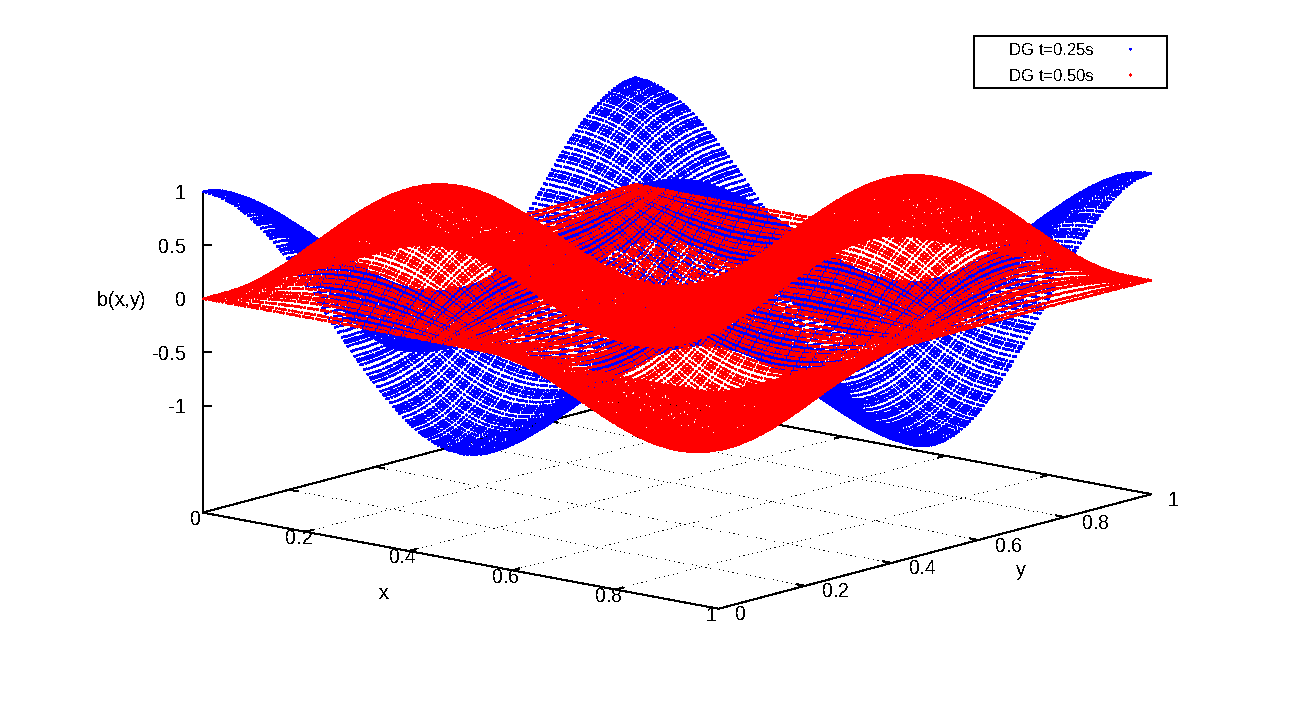
\includegraphics[width=0.90\linewidth]{PNG/Manufacturee/grass_n_x_40_2D.pdf}
        \caption{Vue d'ensemble}
        \label{fig:grass_2d_global}
    \end{subfigure}
    
    \vspace{0.4cm} % Petit espacement vertical entre les deux images
    
    % --- Seconde sous-figure (Vue de tranche / coupe) ---
    \begin{subfigure}{0.96\linewidth}
        \centering
        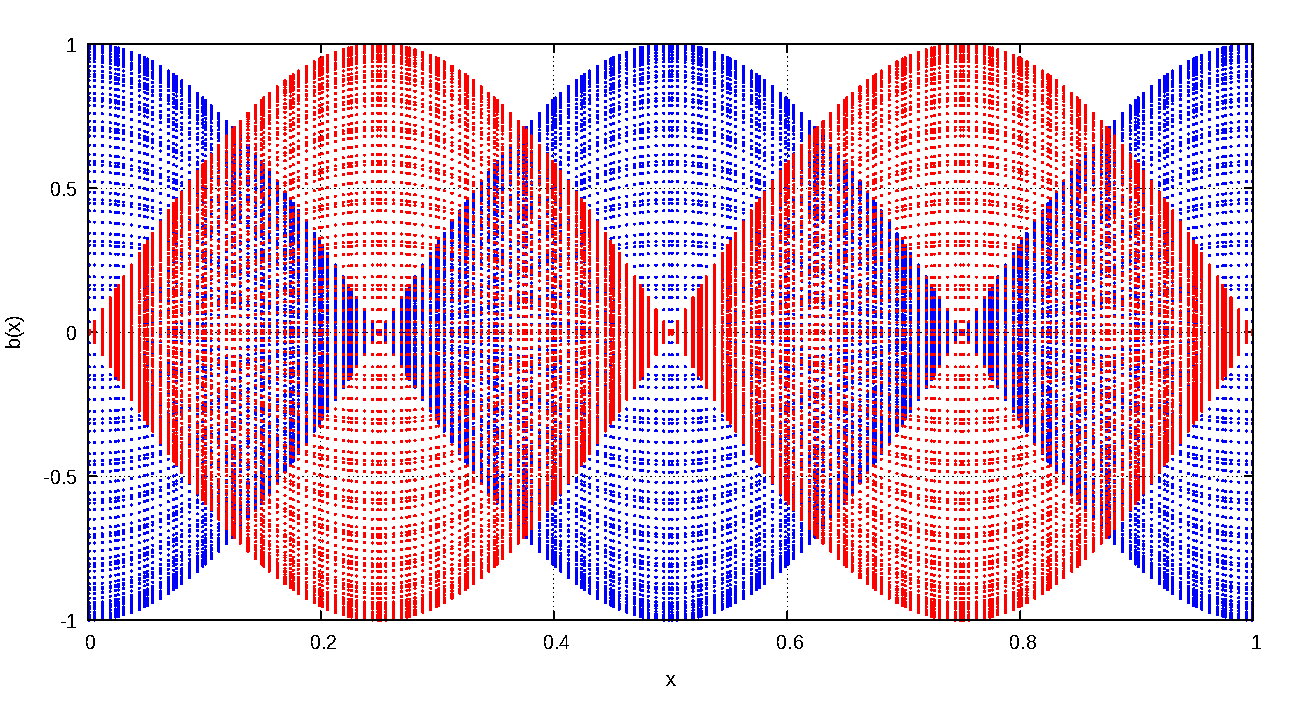
\includegraphics[width=0.80\linewidth]{PNG/Manufacturee/grass_n_x_40_2D_tranche.pdf} % Remplacez par le nom du fichier de profil/tranche
        \caption{Vue de coupe}
        \label{fig:grass_2d_coupe}
    \end{subfigure}
    
    \caption{Cas test 1 -- Représentation des solutions numériques obtenues avec la loi de Grass aux temps $t = \SI{0.25}{\second}$ (en bleu) et $t = \SI{0.5}{\second}$ (en rouge) pour $p = 2$ et $N_e = 40^2$}
    \label{fig:Representation_manufacturee_2D}
\end{figure}

\chapter{Calcul du polynôme caractéristique \texorpdfstring{$\chi_H$}{chi_H}}
\label{annexe:polynome_caracteristique}

Cette annexe présente le développement détaillé du polynôme caractéristique $\chi_H$ de la matrice Jacobienne du système de Saint-Venant-Exner, ainsi que la convergence vers la valeur propre de De Vries utilisée dans le cas test 3.

% Dans ton préambule (ou juste avant l'équation) :
% 1. Placer ceci au tout début de l'annexe (ou dans le préambule)
\allowdisplaybreaks

% 2. Le bloc d'équation scindable
\begin{align}
    \chi_H & = \det \left(\mathbb{H}(\bm{W}) - \lambda \mathbb{I}\right) \notag \\
    & = \begin{vmatrix}
        -\lambda & n_x & n_y & 0 \\
        (gh - u^2) n_x - uv n_y & 2u n_x + v n_y - \lambda & u n_y & gh n_x \\
        (gh - v^2) n_y - uv n_x & v n_x & 2v n_y + u n_x - \lambda & gh n_y \\
        \alpha_n & \beta_n & \gamma_n & -\lambda
    \end{vmatrix} \notag \\
    & = -\lambda \begin{vmatrix}
        2u n_x + v n_y - \lambda & u n_y & gh n_x \\
        v n_x & 2v n_y + u n_x - \lambda & gh n_y \\
        \beta_n & \gamma_n & - \lambda
    \end{vmatrix} \notag \\
    & \quad - n_x \begin{vmatrix}
        (gh - u^2) n_x - uv n_y & u n_y & gh n_x \\
        (gh - v^2) n_y - uv n_x & 2v n_y + u n_x - \lambda & gh n_y \\
        \alpha_n & \gamma_n & -\lambda
    \end{vmatrix} \notag \\
    & \quad + n_y \begin{vmatrix}
        (gh - u^2) n_x - uv n_y & 2u n_x + v n_y - \lambda & gh n_x \\
        (gh - v^2) n_y - uv n_x & v n_x & gh n_y \\
        \alpha_n & \beta_n & -\lambda
    \end{vmatrix} \notag \\
    & = - \lambda (2u n_x + v n_y - \lambda) \begin{vmatrix}
        2v n_y + u n_x - \lambda & gh n_y \\
        \gamma_n & -\lambda
    \end{vmatrix}
    + \lambda u n_y \begin{vmatrix}
        v n_x & gh n_y \\
        \beta_n & - \lambda
    \end{vmatrix} \notag \\
    & \quad - \lambda gh n_x \begin{vmatrix}
        v n_x & 2v n_y + u n_x - \lambda \\
        \beta_n & \gamma_n
    \end{vmatrix} \notag \\
    & \quad -((gh - u^2) n_x - uv n_y) n_x \begin{vmatrix}
        2v n_y + u n_x - \lambda & gh n_y \\
        \gamma_n & -\lambda
    \end{vmatrix} \notag \\
    & \quad + u n_x n_y \begin{vmatrix}
        (gh - v^2) n_y - uv n_x & gh n_y \\
        \alpha_n & -\lambda
    \end{vmatrix} \notag \\
    & \quad - gh n_x^2 \begin{vmatrix}
        (gh - v^2) n_y - uv n_x & 2v n_y + u n_x -\lambda \\
        \alpha_n & \gamma_n
    \end{vmatrix} \notag \\
    & \quad + ((gh - u^2) n_x - uv n_y) n_y \begin{vmatrix}
        v n_x & gh n_y \\
        \beta_n & - \lambda
    \end{vmatrix} \notag \\
    & \quad - (2u n_x + v n_y - \lambda) n_y \begin{vmatrix}
        (gh - v^2) n_y - uv n_x & gh n_y \\
        \alpha_n & -\lambda
    \end{vmatrix} + gh n_x n_y \begin{vmatrix}
        (gh - v^2) n_y - uv n_x & v n_x \\
        \alpha_n & \beta_n
    \end{vmatrix} \notag \\
    & = \lambda (2u n_x + v n_y - \lambda) \left[ \lambda (2v n_y + u n_x - \lambda) + \gamma_n gh n_y \right] + \lambda u n_y \left[ - \lambda v n_x - \beta_n gh n_y \right] \notag \\
    & \quad - \lambda gh n_x \left[ \gamma_n v n_x - \beta_n (2v n_y + u n_x - \lambda) \right] \notag \\
    & \quad - ((gh - u^2) n_x - uv n_y) n_x \left[ - \lambda(2v n_y + u n_x - \lambda) - \gamma_n gh n_y \right] \notag \\
    & \quad + u n_x n_y \left[ - \lambda((gh - v^2) n_y - uv n_x) - \alpha_n gh n_y \right] \notag \\
    & \quad - gh n_x^2 \left[ \gamma_n ((gh - v^2) n_y - uv n_x) - \alpha_n (2v n_y + u n_x - \lambda) \right] \notag \\
    & \quad + ((gh - u^2) n_x - uv n_y) n_y \left[ -\lambda v n_x - \beta_n gh n_y \right] \notag \\
    & \quad - (2u n_x + v n_y - \lambda) n_y \left[ -\lambda((gh - v^2) n_y - uv n_x) - \alpha_n gh n_y \right] \notag \\
    & \quad + gh n_x n_y \left[ \beta_n ((gh - v^2) n_y - uv n_x) - \alpha_n v n_x \right] \notag \\
    \chi_H & = \lambda^4 - 3u_n \lambda^3 + \left[ 3 u_n^2 -gh(1 + \beta_n n_x + \gamma_n n_y) \right] \lambda^2 \notag \\
    & \quad - \left[ u_n(u_n^2 - gh) + gh \left( \alpha_n - u_n(\beta_n n_x + \gamma_n n_y) + (u n_y - v n_x)(\beta_n n_y - \gamma_n n_x) \right) \right] \lambda \notag \\
    & \quad + gh u_n \left[ \alpha_n + (\beta_n n_y - \gamma_n n_x)(u n_y - v n_x) \right] \label{eq:polynome_exner}
\end{align}

De plus, le polynôme caractéristique \eqref{eq:Polynome_caracteristique} nous permet de retrouver la valeur propre de De Vries en 1D et d'étendre cette dernière en 2D. \\
Pour ce faire, comme l'échelle de temps de l'évolution de la bathymétrie est lente devant la dynamique de l'eau en régime sous-critique, l'idée de De Vries \cite{vries1965considerations} est d'effectuer un développement limité à l'ordre 1 autour de $\lambda = 0$. \\
Ainsi, il vient
\begin{equation}
    - \left[ u_n(u_n^2 - gh) + gh \left( \alpha_n - u_n \delta_n + u_t \delta_t \right) \right] \lambda_\text{DV} + gh u_n \left[ \alpha_n + u_t \delta_t \right] = 0
\end{equation}
soit
\begin{equation}
    \lambda_\text{DV} = \frac{\left( \alpha_n + u_t \delta_t \right) u_n}{-u_n \left( 1 - \text{Fr}_n^2 \right) + \alpha_n + u_t \delta_t - u_n \delta_n}
\end{equation}
En particulier, si nous utilisons la loi de Grass en 2D, alors
\begin{equation}
    \begin{aligned}
        G_n & = A_G \frac{1}{h^{m_G}} \| \bm{q} \|^{m_G - 1} q_n \\
        \alpha_n & = -m_G A_G \frac{1}{h^{m_G + 1}} \| \bm{q} \| q_n = - m_G \frac{1}{h} G_n \\
        \beta_n & = A_G \frac{1}{h} \| \bm{u} \|^{m_G - 1} \left( n_x + (m_G - 1) \frac{u}{\| \bm{u} \|^2} u_n \right) \\
        \gamma_n & = A_G \frac{1}{h} \| \bm{u} \|^{m_G - 1} \left( n_y + (m_G - 1) \frac{v}{\| \bm{u} \|^2} u_n \right) \\
    \end{aligned}
\end{equation}
D'où
\begin{equation}
    \begin{aligned}
        \delta_n & = A_G \frac{1}{h} \| \bm{u} \|^{m_G - 1} \left( 1 + (m_G - 1) \frac{u_n^2}{\| \bm{u} \|^2} \right) = \frac{G_n}{h u_n} \left( 1 + (m_G - 1) \frac{u_n^2}{\| \bm{u} \|^2} \right) \\
        \delta_t & = A_G \frac{1}{h} \| \bm{u} \|^{m_G - 1} (m_G - 1) \frac{u_t}{\| \bm{u} \|^2} u_n = \frac{G_n}{h u_n} (m_G - 1) \frac{u_n u_t}{\| \bm{u} \|^2}
    \end{aligned}
\end{equation}
Par conséquent,
\begin{equation}
    \alpha_n + u_t \delta_t = - u_n \delta_n
\end{equation}
On obtient alors la valeur propre de De Vries en 2D pour la loi de Grass sous la forme
\begin{equation}
    \lambda_\text{DV} = \frac{\delta_n}{1 - \text{Fr}_n^2 + 2 \delta_n} u_n
\end{equation}
En outre, pour un écoulement 1D, $\delta_n = \beta_n = \beta$ et $u_n = u$, d'où
\begin{equation}
    \lambda_\text{DV,1D} = \frac{\beta}{1 - \text{Fr}^2 + 2 \beta} u
\end{equation}
Or, comme le flux de sédiments $G$ est petit devant le débit d'eau $q$ lorsque l'écoulement est en régime sous-critique et que
\begin{equation}
    \beta \sim m_G \frac{G}{q} \ll 1 - \text{Fr}^2
\end{equation}
nous retrouvons la valeur propre de De Vries en 1D pour la loi de Grass \cite{fernandez2025third, vries1965considerations}
\begin{equation}
    \lambda_\text{DV,1D} = \frac{\beta}{1 - \text{Fr}^2} u
\end{equation}
Enfin, comme chaque terme de perturbation hydro-sédimentaire du polynôme caractéristique $\chi_H$ est proportionnel au ratio $G_n/q_n$, nous pouvons en première approximation conserver les trois autres valeurs propres usuelles issues de $(\mathcal{SW})$. \\
Autrement, si nous souhaitions trouver les racines exactes, il faudrait employer une méthode itérative pour chaque face à chaque sous-pas de temps. Ce processus est très coûteux d'une part, et rien ne garantit sa convergence vers les vraies racines d'autre part. \\
Cependant, Fernandez-Nieto \textit{et al.} \cite{fernandez2025third} ont montré que les approximations de De Vries ne sont valables que pour des nombres de Froude inférieurs à $0.7$ environ. Au-delà, les valeurs propres sont sur-estimées, entraînant une sur-diffusion numérique. En ce sens, il serait possible d'implémenter une méthode itérative dès lors que le nombre de Froude local $\text{Fr}_n > 0.7$.

\end{appendices}

\newpage
\section*{Remerciements}

Ce travail a bénéficié d'un financement dans le cadre du projet HydrauMATH.

\addcontentsline{toc}{chapter}{Bibliographie}
\bibliographystyle{plain}
\bibliography{references}

\end{document}